%%%%%%%%%%%%%%%%%%%%%%%%%%%%%%%%%%%%%%%%%
% Masters/Doctoral Thesis 
% LaTeX Template
% Version 2.4 (22/11/16)
%
% This template has been downloaded from:
% http://www.LaTeXTemplates.com
%
% Version 2.x major modifications by:
% Vel (vel@latextemplates.com)
%
% This template is based on a template by:
% Steve Gunn (http://users.ecs.soton.ac.uk/srg/softwaretools/document/templates/)
% Sunil Patel (http://www.sunilpatel.co.uk/thesis-template/)
%
% Template license:
% CC BY-NC-SA 3.0 (http://creativecommons.org/licenses/by-nc-sa/3.0/)
%
%%%%%%%%%%%%%%%%%%%%%%%%%%%%%%%%%%%%%%%%%

%----------------------------------------------------------------------------------------
%	PACKAGES AND OTHER DOCUMENT CONFIGURATIONS
%----------------------------------------------------------------------------------------

\documentclass[
11pt, % The default document font size, options: 10pt, 11pt, 12pt
%oneside, % Two side (alternating margins) for binding by default, uncomment to switch to one side
english, % ngerman for German
onehalfspacing, % Single line spacing, alternatives: onehalfspacing or doublespacing
%draft, % Uncomment to enable draft mode (no pictures, no links, overfull hboxes indicated)
%nolistspacing, % If the document is onehalfspacing or doublespacing, uncomment this to set spacing in lists to single
%liststotoc, % Uncomment to add the list of figures/tables/etc to the table of contents
%toctotoc, % Uncomment to add the main table of contents to the table of contents
%parskip, % Uncomment to add space between paragraphs
%nohyperref, % Uncomment to not load the hyperref package
%headsepline, % Uncomment to get a line under the header
%chapterinoneline, % Uncomment to place the chapter title next to the number on one line
%consistentlayout, % Uncomment to change the layout of the declaration, abstract and acknowledgements pages to match the default layout
]{MastersDoctoralThesis} % The class file specifying the document structure

\usepackage[utf8]{inputenc} % Required for inputting international characters
\usepackage[T1]{fontenc} % Output font encoding for international characters
\usepackage{fontspec} % Better font handling

\usepackage[newfloat]{minted} % Code Highlighting
\usepackage{caption}
\usepackage{tcolorbox}
\usepackage{etoolbox}

\newenvironment{code}{\captionsetup{type=listing}}{}
\SetupFloatingEnvironment{listing}{name=Snippet}

\BeforeBeginEnvironment{minted}{\begin{tcolorbox}}%
\AfterEndEnvironment{minted}{\end{tcolorbox}}%


\setmainfont{Palatino Linotype}
\setmonofont{Consolas}

\usepackage[backend=bibtex,style=numeric,natbib=true]{biblatex} % Use the bibtex backend with the authoryear citation style (which resembles APA)

\addbibresource{bibliography.bib} % The filename of the bibliography

\usepackage[autostyle=true]{csquotes} % Required to generate language-dependent quotes in the bibliography

\newcommand*\justify{%
    \fontdimen2\font=0.4em% interword space
    \fontdimen3\font=0.2em% interword stretch
    \fontdimen4\font=0.1em% interword shrink
    \fontdimen7\font=0.1em% extra space
    \hyphenchar\font=`\-% allowing hyphenation
}


%----------------------------------------------------------------------------------------
%	MARGIN SETTINGS
%----------------------------------------------------------------------------------------

\geometry{
	paper=letterpaper, % Change to letterpaper for US letter
	inner=2.5cm, % Inner margin
	outer=3.8cm, % Outer margin
	bindingoffset=.5cm, % Binding offset
	top=3.5cm, % Top margin
	bottom=3cm, % Bottom margin
	%showframe, % Uncomment to show how the type block is set on the page
}

%----------------------------------------------------------------------------------------
%	THESIS INFORMATION
%----------------------------------------------------------------------------------------

\thesistitle{A Big Data Architecture: from Ingestion to Analytics} % Your thesis title, this is used in the title and abstract, print it elsewhere with \ttitle
\supervisor{Dott. Luca \textsc{Oneto}} % Your supervisor's name, this is used in the title page, print it elsewhere with \supname
\examiner{} % Your examiner's name, this is not currently used anywhere in the template, print it elsewhere with \examname
\degree{Corso di Studio in Ingegneria Informatica} % Your degree name, this is used in the title page and abstract, print it elsewhere with \degreename
\author{Federico \textsc{D'Ambrosio}, Edoardo \textsc{Ferrante}} % Your name, this is used in the title page and abstract, print it elsewhere with \authorname
\addresses{} % Your address, this is not currently used anywhere in the template, print it elsewhere with \addressname

\subject{Data Analysis} % Your subject area, this is not currently used anywhere in the template, print it elsewhere with \subjectname
\keywords{} % Keywords for your thesis, this is not currently used anywhere in the template, print it elsewhere with \keywordnames
\university{{Università degli studi di Genova}} % Your university's name and URL, this is used in the title page and abstract, print it elsewhere with \univname
\department{\href{http://www.dibris.unige.it/}{Dibris}} % Your department's name and URL, this is used in the title page and abstract, print it elsewhere with \deptname
\group{\href{http://researchgroup.university.com}{Research Group Name}} % Your research group's name and URL, this is used in the title page, print it elsewhere with \groupname
\faculty{\href{http://www.informatica.ingegneria.unige.it/}{Ingegneria Informatica}} % Your faculty's name and URL, this is used in the title page and abstract, print it elsewhere with \facname

\AtBeginDocument{
\hypersetup{pdftitle=\ttitle} % Set the PDF's title to your title
\hypersetup{pdfauthor=\authorname} % Set the PDF's author to your name
\hypersetup{pdfkeywords=\keywordnames} % Set the PDF's keywords to your keywords
}

\begin{document}
\hypersetup{colorlinks, urlcolor=blue, linkcolor=blue}

\frontmatter % Use roman page numbering style (i, ii, iii, iv...) for the pre-content pages

\pagestyle{plain} % Default to the plain heading style until the thesis style is called for the body content

%----------------------------------------------------------------------------------------
%	TITLE PAGE
%----------------------------------------------------------------------------------------

\begin{titlepage}
%\linespread{1.5}
\thispagestyle{empty}
\begin{center}
	
\includegraphics[width=0.2\linewidth]{Figures/unige.eps}
\end{center}

\begin{center}
	\LARGE\sc
	\univname\\
	
	\vspace{0.5cm}
	\large
	\degreename\\
\end{center}

\begin{center}
	\small
	Tesi di Laurea per il conseguimento del titolo di\\
	Dottore Magistrale in Ingegneria Informatica\\
\end{center}

\vfill

\begin{center} 
	\LARGE
	{\bf \ttitle}\\
	\vspace{0.5cm}
	\large
	\authorname\\
	\vspace{0.5cm}
	\small
	Dicembre 2017
\end{center}

\vfill

\begin{tabular}{lll}%
	{\em Relatore}:	& Prof.	& Luca Oneto\\
	{\em Relatore}:	& Prof.	& Davide Anguita\\
\end{tabular} 

\hfill


\end{titlepage}


%----------------------------------------------------------------------------------------
%	QUOTATION PAGE
%----------------------------------------------------------------------------------------

%\vspace*{0.2\textheight}

%\noindent\enquote{\itshape Thanks to my solid academic training, today I can write hundreds of words on virtually any topic without possessing a shred of information, which is how I got a good job in journalism.}\bigbreak

%\hfill Dave Barry

%----------------------------------------------------------------------------------------
%	ABSTRACT PAGE
%----------------------------------------------------------------------------------------

\begin{abstract}
\addchaptertocentry{\abstractname} % Add the abstract to the table of contents
This thesis aims to analyse the many components required for a Big Data infrastructure and to identify the ideal ones among the state-of-the-art products in the ever renewing environment of Big Data analytics, amidst the context of Business Intelligence and Data Driven Decision Making for industries.
Real world applications need, in this context, a well defined infrastructure, scalable, flexible with interchangeable components as the use case needs. In order to show this, we applied the aforementioned concepts in an air traffic monitoring application, a service similar to those provided by FlightRadar or FlightAware, through the implementation of a data processing pipeline, starting from the ingestion of the raw data, ending with the processing and visualization of analytics.
The results show that the tools available are powerful and customizable and allow for a wide range of useful implementations ranging from reporting systems and real time monitoring to decision support applications.
\end{abstract}

%----------------------------------------------------------------------------------------
%	ACKNOWLEDGEMENTS
%----------------------------------------------------------------------------------------

\begin{acknowledgements}
\addchaptertocentry{\acknowledgementname} % Add the acknowledgements to the table of contents
The acknowledgments and the people to thank go here, don't forget to include your project advisor\ldots
\end{acknowledgements}

%----------------------------------------------------------------------------------------
%	LIST OF CONTENTS/FIGURES/TABLES PAGES
%----------------------------------------------------------------------------------------

\tableofcontents % Prints the main table of contents


%----------------------------------------------------------------------------------------
%	DEDICATION
%----------------------------------------------------------------------------------------

\dedicatory{For/Dedicated to/To my\ldots} 

%----------------------------------------------------------------------------------------
%	THESIS CONTENT - CHAPTERS
%----------------------------------------------------------------------------------------

\mainmatter % Begin numeric (1,2,3...) page numbering

\pagestyle{thesis} % Return the page headers back to the "thesis" style

% Include the chapters of the thesis as separate files from the Chapters folder
% Uncomment the lines as you write the chapters


\chapter{Introduzione}

\section{Big Data: che cosa sono?}

\section{A Big Data Infrastructure}\label{Chapter2}

\subsection{Hardware}

\subsection{Data \& Cluster Management}

\subsection{Data Access}

\subsection{Data Quality}

\subsection{Data Processing}

\subsection{Data Ingestion}

\subsection{Data Visualization}

\subsection{Management \& Operations}

\subsection{Security}
 
\chapter{Data Management \& Data Access}

\section{HDFS}

The Hadoop Distributed File System, or HDFS for short, is a distributed File System engineered to run on any kind of hardware and to be easily scalable into huge clusters. Originally developed for Apache Nutch is now part of the Hadoop project, providing high fault-tolerance thanks to data replication and high throughput access to application data, making it suitable for Big Data applications.

\subsection{Architecture} 

HDFS has a master-slave architecture, comprised of two main components: a single \textbf{NameNode} which functions as a master and is in charge of the File System namespace management and the access control on its data by the clients and a list of \textbf{DataNodes} spread among the cluster's machines which handle the storage on the node they run on.\newline
HDFS interface, managed by the \textbf{NameNode} exposes a File System namespace and allows users to store data in files within a directory-based hierarchy, much like the regular File Systems used in general purpose machines; under the surface the file is split in one or more blocks which are then stored on a subset of \textbf{DataNodes} called rack.\newline The \textbf{NameNode} stores the metadata of the content of the whole File System and is responsible for the File System namespace operations over the files and directories and determines how blocks are mapped to the \textbf{DataNodes}.
The \textbf{DataNodes} serve the read and write requests sent by the File System's clients and can perform basic operations on the block (creation, deletion, copy) when so instructed by the \textbf{NameNode}.

\subsection{Replication} 

Exposing a File System built upon a cluster of many machines requires the technology to be reliable in case of a malfunction, since the chance of failure of the whole system is inherently greater if its functions depend on any of the single machines that comprise it. \newline Therefore to make sure that data is always available to clients, whenever a file is stored on the File System namespace and the \textbf{NameNode} chooses where to store the single blocks, it actually store the same block on more than one \textbf{DataNode} (the number depends on a configuration aptly named Replication Factor), in such a way that if any of those nodes become inaccessible for any reason, among all the others will always be a reachable copy of each block stored on it.\newline Secondly, the \textbf{NameNode} must always be available, therefore the HDFS provides a \textbf{Secondary NameNode}.

\subsection{Persistence}

The File System metadata, as previously stated, is managed by the \textbf{NameNode}. The \textbf{NameNode} uses a log to store persistently all the changes to these metadata, such as changing the replication factor, creating a new file, renaming an old one; the log, called EditLog, is stored in the host machine's File System. Similarly the state of the File System is stored on the machine's File System in a file called FsImage.\newline
In case of HDFS failure, on restart the \textbf{NameNode} will load in memory the FsImage and then apply all the transactions stored on EditLog, to return to the last safe state it was before failure.
\newline
If no failures occur and the \textbf{NameNode} is not restarted, FsImage will become stale while EditLog's size will continue to increase to unmanageable size, to cope with this problem, HDFS uses a \textbf{Secondary NameNode} whose object is to query EditLogs to the \textbf{Primary NameNode} at regular intervals, to update its own copy of FsImage accordingly and to then send its copy to the \textbf{Primary NameNode}.

\subsection{Robustness}

HDFS is designed to be reliable in the event of the three most common failures: \textbf{NameNode} failures, \textbf{DataNode} failure and network failures.

Each \textbf{DataNode} sends a heartbeat regularly to the \textbf{NameNode} to prove its liveness, the latter considers the formers without recent heartbeats dead and stop sending read and write requests to them until a new heartbeat arrives.\newline
While \textbf{DataNodes} failures may cause them to be dead, Network failures can cause alive \textbf{DataNodes} to lose their heartbeats and be considered dead.\newline
Whatever the root of the problem, the \textbf{NameNode} tracks the blocks that are now under replicated and marks them to be replicated as soon as it has available space on a machine that doesn't already have a copy of them.\newline
Checksums for each block of stored files make sure that corruption caused by faults in Nodes are spotted and their corrupted blocks rejected.\newline
As for \textbf{NameNode} problems, the secondary \textbf{Secondary NameNode} manages a consistent copy of FsImage and EditLog that functions as a backup in case of the corruption of the original ones. Nevertheless the \textbf{NameNode} is a single point of failure in the whole system; this is solved through High Availability, by providing a perfect another \textbf{NameNode}, which serves as a \textbf{Secondary NameNode} during downtime and as a \textbf{Primary NameNode} if the main one is not available.

\pagebreak
\section{YARN} \label{YARN}

\textbf{YARN (Yet Another Resource Negotiator)} is Hadoop's cluster and resource manager, whose fundamental idea is to split up the functionalities of resource management and job scheduling and monitoring into separate daemons: a global \textbf{Resource Manager (RM)} and per-application, either a single job or a DAG of jobs, \textbf{Application Master (AM)}.
\newline\newline
The \textbf{Resource Manager}, together with the \textbf{Node Manager (NM)}, forms the data-computation framework: the first one is the ultimate authority that arbitrates resources among all the applications in the system, while the other is the per-machine framework agent who is responsible for containers, monitoring their resource usage and reporting it to the Resource Manager.
\newline\newline
The per-application Application Master is, in effect, a framework specific library and is tasked with negotiating resources from the Resource Manager and working with the Node Manager(s) to execute and monitor the tasks.

\subsection{Resource Manager}

The \textbf{Resource Manager}, the master component in YARN architecture, has two main components: the Scheduler and the Applications Manager.

The \textbf{Scheduler} is responsible for allocating resources to the various running applications subject to familiar constraints of capacities, queues etc. It performs no monitoring or tracking of status for the application and offers no guarantees about restarting failed tasks either due to application failure or hardware failures. 

Scheduling is performed based on the abstract notion of a Container incorporating elements such as memory, CPU, disk, network etc. which represent the resource requirements of the applications. It has a pluggable policy which is responsible for partitioning the cluster resources among the various queues, applications etc. The current schedulers such as the \textit{Capacity Scheduler} and the \textit{Fair Scheduler} would be some examples of plug-ins.

The \textbf{Applications Manager} is responsible for accepting job-submissions, negotiating the first container for executing the application specific Application Master and provides the service for restarting the Application Master container on failure. The per-application Application Master has the responsibility of negotiating appropriate resource containers from the Scheduler, tracking their status and monitoring for progress.

YARN supports the notion of resource reservation via a \textbf{Reservation System}, that allows users to specify a profile of resources over-time and temporal constraints (e.g., deadlines), and reserve resources to ensure the predictable execution of important jobs. The Reservation System tracks resources over-time, performs admission control for reservations, and dynamically instruct the underlying scheduler to ensure that the reservation is fulfilled.

\subsubsection{Schedulers}

There are two possible schedulers that can be used in a YARN cluster: \textbf{Capacity Scheduler} and \textbf{Fair Scheduler}. While the first one allows for multiple-tenants to securely share a large cluster by allocating resources in a timely manner under capacity constraints, the other allows for YARN applications to share cluster resources fairly.

\paragraph{Capacity Scheduler}

The Capacity Scheduler is designed to run Hadoop applications as a shared, multi-tenant cluster in an operator-friendly manner while maximizing the throughput and the utilization of the cluster.

Traditionally each organization has its own private set of computing resources that have sufficient capacity to meet the organization’s Service Level Agreement under peak or near-peak conditions. This generally leads to poor average utilization and overhead of managing multiple independent clusters, one per each organization. Sharing clusters between organizations is a cost-effective manner of running large Hadoop installations since this allows them to reap benefits of economies of scale without creating private clusters. However, organizations may be concerned about sharing a cluster because they are worried about others using the resources that are critical for their applications needs.

The Capacity Scheduler is designed to allow sharing a large cluster while giving each organization capacity guarantees. The central idea is that the available resources in the Hadoop cluster are shared among multiple organizations who collectively fund the cluster based on their computing needs. There is an added benefit that an organization can access any excess capacity not being used by others. This provides elasticity for the organizations in a cost-effective manner.

Sharing clusters across organizations necessitates strong support for multi-tenancy since each organization must be guaranteed capacity and safe-guards to ensure the shared cluster is impervious to a single rogue application or user, or sets thereof. The Capacity Scheduler provides a stringent set of limits to ensure that a single application or user or queue cannot consume disproportionate amount of resources in the cluster. Also, the Capacity Scheduler provides limits on initialized and pending applications from a single user and queue to ensure fairness and stability of the cluster.

The primary abstraction provided by the Capacity Scheduler is the concept of queues. These queues are typically set up by administrators to reflect the economics of the shared cluster.

The Capacity Scheduler supports the following features:

\begin{itemize}

\item \textbf{Hierarchical Queues} - Hierarchy of queues is supported to ensure resources are shared among the sub-queues of an organization before other queues are allowed to use free resources, thereby providing more control and predictability.

\item \textbf{Capacity Guarantees} - Queues are allocated a fraction of the capacity of the grid in the sense that a certain capacity of resources will be at their disposal. All applications submitted to a queue will have access to the capacity allocated to the queue. Administrators can configure soft limits and optional hard limits on the capacity allocated to each queue.

\item \textbf{Security} - Each queue has strict ACLs\footnote{ACL: Access Control List, a data structure holding the permissions on an object for each user.} which controls which users can submit applications to individual queues. Also, there are safe-guards to ensure that users cannot view and/or modify applications from other users. Also, per-queue and system administrator roles are supported.

\item \textbf{Elasticity} - Free resources can be allocated to any queue beyond its capacity. When there is demand for these resources from queues running below capacity at a future point in time, as tasks scheduled on these resources complete, they will be assigned to applications on queues running below the capacity (pre-emption is also supported). This ensures that resources are available in a predictable and elastic manner to queues, thus preventing artificial silos of resources in the cluster which helps utilization.

\item \textbf{Multi-tenancy} - Comprehensive set of limits are provided to prevent a single application, user and queue from monopolizing resources of the queue or the cluster as a whole to ensure that the cluster isn't overwhelmed.

\item \textbf{Operability}
    \begin{itemize}
    \item \textbf{Runtime Configuration} - The queue definitions and properties such as capacity and ACLs can be changed, at runtime, by administrators in a secure manner to minimize disruption to users. Also, a console is provided for users and administrators to view current allocation of resources to various queues in the system. Administrators can add additional queues at runtime, but queues cannot be deleted at runtime.
    
    \item \textbf{Drain applications} - Administrators can stop queues at runtime to ensure that while existing applications run to completion, no new applications can be submitted. If a queue is in STOPPED state, new applications cannot be submitted to itself or any of its child queues. Existing applications continue to completion, thus the queue can be drained gracefully. Administrators can also start the stopped queues.
    \end{itemize}

\item \textbf{Queue Mapping based on User or Group} - This feature allows users to map a job to a specific queue based on the user or group.

\item \textbf{Priority Scheduling} - This feature allows applications to be submitted and scheduled with different priorities. Higher integer value indicates higher priority for an application. Currently Application priority is supported only for FIFO\footnote{FIFO: First In First Out, a policy for the executions of jobs, the first job to come is the first to be served.} ordering policy.

\end{itemize}

\paragraph{Fair Scheduler}

Fair scheduling is a method of assigning resources to applications such that all of them get, on average, an equal share of resources over time. Hadoop is capable of scheduling multiple resource types:  the Fair Scheduler bases, by default, scheduling fairness decisions only on memory, but it can be configured to schedule with both memory and CPU. When there is a single application running, it uses the entire cluster, and when other applications are submitted, resources that free up are assigned to them, so that each one eventually gets roughly the same amount of resources. Unlike the default Hadoop scheduler, which forms a queue of applications, this lets short apps finish in reasonable time while not starving long-lived apps. It is also a reasonable way to share a cluster between a number of users. Finally, fair sharing can also work with priorities, which are used as weights to determine the fraction of total resources that each application should get.

The scheduler organizes apps further into "queues", and shares resources fairly between these queues. By default, all users share a single queue, named “default”. If an app specifically lists a queue in a container resource request, the request is submitted to that queue. It is also possible to assign queues based on the user name included with the request through configuration. Within each queue, a scheduling policy is used to share resources between the running apps. The default is memory-based fair sharing, but FIFO and multi-resource with Dominant Resource Fairness can also be configured. Queues can be arranged in a hierarchy to divide resources and configured with weights to share the cluster in specific proportions.

In addition to providing fair sharing, the Fair Scheduler allows assigning guaranteed minimum shares to queues, useful for ensuring that certain users, groups or production applications always get sufficient resources. When a queue contains apps, it gets at least its minimum share, but when the queue does not need its full guaranteed share, the excess is split between other running apps. This lets the scheduler guarantee capacity for queues while utilizing resources efficiently when these queues don’t contain applications.

The Fair Scheduler lets all apps run by default, but it is also possible to limit the number of running apps per user and per queue, useful when a user must submit hundreds of apps at once, or in general to improve performance if running too many apps at once would cause too much intermediate data to be created or too much context-switching. Limiting the apps does not cause any subsequently submitted apps to fail, only to wait in the scheduler’s queue until some of the user’s earlier apps finish.

The Fair Scheduler, just like the Capacity Scheduler, supports hierarchical queues. All queues descend from a queue named “root”. Available resources are distributed among the children of the root queue in the typical fair scheduling fashion. Then, the children distribute the resources assigned to them to their children in the same fashion. Applications may only be scheduled on leaf queues. Queues can be specified as children of other queues by placing them as sub-elements of their parents in the fair scheduler allocation file.

Additionally, the fair scheduler allows setting a different custom policy for each queue to allow sharing the queue’s resources in any which way the user wants: FifoPolicy, FairSharePolicy (default), and DominantResourceFairnessPolicy are built-in and can be readily used, but a custom policy can be specified by extending \texttt{SchedulingPolicy} class. 

\subsubsection{Fault tolerance \& High Availability}

The Resource Manager is the central authority that manages resources and schedules applications running on YARN. Hence, it is potentially a single point of failure in a YARN cluster. 

They are thus needed functionalities that provide for down-time invisibility to end-users, keeping the RM functioning across restarts and remedying in case of node failures.

\paragraph{Non-work-preserving RM restart} RM will save the application metadata, together with credentials like security keys and tokens, when clients submit an application in a pluggable state-store, storing its status and diagnostics at completion. In case of RM outage, as long as the required information is available in the state-store, at restart, the RM can pick up the application metadata and re-submit the applications if they weren't already completed (failed, killed, or finished) before RM went down.

During the down-time of RM, Node Managers and clients will keep polling RM until it comes up. Once it does, a re-sync command is sent by the RM, killing all NM's managed containers, re-registering with RM, shutting down this way all the Application Masters. After RM restarts and loads all the application metadata, it will create a new attempt (i.e. Application Master) for each application not yet completed, re-kicking that application as usual.

\paragraph{Work-preserving RM restart} This type of restart focuses on re-constructing the running state of RM by combining the container status from Node Managers and container requests from Application Masters on restart: running applications won't be killed after RM restarts, and so applications will not lose their work because of RM outage. 

RM ensures the persistence of application state, reloading it on recovery and re-constructing the entire running state of the YARN cluster, whose major information comes from the RM scheduler which keeps track of all containers' life-cycle, applications' headroom and resource requests and queues' resource usage. 
Applications can simply re-sync back with RM and resume from where they were left off: RM recovers its own running state by taking advantage of the containers statuses sent from all NMs on re-registration, reconstructing the container instances and the associated applications' scheduling status by absorbing this information. 

In the meantime, AM needs to re-send the resource requests to RM because RM may lose the unfulfilled requests when it shuts down.

\paragraph{High Availability} Resource Manager HA is realized through an Active/Standby architecture: at any point of time, one of the RMs is Active, and one or more RMs are in Standby mode waiting to take over should anything happen to the Active. The trigger to transition-to-active comes from either the admin (through CLI) or through the integrated failover-controller when automatic-failover is enabled. When automatic fail-over is not enabled, admins have to manually transition one of the RMs to Active, using the \verb|yarn rmadmin| CLI, first transitioning the Active-RM to Standby and then the Standby-RM to Active.

In order to guarantee automatic fail-over, it's possible to use both an existing \textbf{Zookeeper} cluster or the embedded \verb|ActiveStandbyElector|, acting as a failure detector and leader elector instead of a separate Zookeeper FailoverController daemon, to decide which RM should be the Active: when the Active goes down or becomes unresponsive, another RM is automatically elected to be the Active, taking then over.

When there are multiple RMs, the configuration (\verb|yarn-site.xml|) used by clients and nodes is expected to list all the RMs. Clients, Application Masters and Node Managers try connecting to the RMs in a round-robin fashion until they hit the Active RM. If the Active goes down, they resume the round-robin polling until they hit the “new” Active. This retry logic can be overridden by a user-specified fail-over provider.

\subsection{Node Manager \& Application Manager}

\pagebreak
\section{SQL: Hive}

Apache Hive is a relational database for Big Data, developed as a part of the Hadoop environment to provide fast access to huge data sets through its own query language, \textbf{HiveQL}, and through several possible execution engines such as Apache Tez, MapReduce and Apache Spark. Hive, as of recently, added  support for ACID transactions, making it viable as a data storage for more complex endeavours, including streaming applications.

\subsection{Components}

Hive architecture can be divided in five main components:

\begin{itemize}
    \item \textbf{Shell/UI}: Beeline is the frontend tool for interactive querying on the database. Hive supports connections via its own JDBC driver, allowing easy integration with clients and user applications.
    \item \textbf{Driver}: The component which receives the queries. This component implements the notion of session handles and provides execute and fetch APIs\footnote{API: Application Programming Interface, a set of functions and protocols provided to developers.} modeled on JDBC/ODBC interfaces.
    \item \textbf{Metastore}: It stores metadata about HDFS file locations and the table schemas, but also column and column type information and the serializers and deserializers necessary to read and write data.
    \item \textbf{Compiler}: It manages query parsing, planning and optimization, does semantic analysis on the different query blocks and query expressions generating, eventually, an execution plan with the help of the table and partition metadata looked up from the metastore. For what concerns the parsing, HiveQL is a SQL extension, compliant with the SQL:2011 standard.
    \item \textbf{Execution Engine}: Hive uses Apache Tez as a default execution engine  which allows low latency querying through its LLAP (Low Latency Analytical Processing) daemons: persistent processes running on YARN enabling the system to avoid the overhead caused by the container deployment for query executions. Other execution engines usable by Hive are, as already mentioned, MapReduce and Spark. The first one is needed, as of Hive 2.1, in order to use Hive Streaming API, while the other uses its own LLAP daemons, similarly to Tez, and still lags behind, performance wise.
\end{itemize}

\subsection{Hive Low Latency Processing on Tez}

Starting from Hive2, OLAP, OnLine Analytical Processing support has been introduced as default mode for query execution on top of Apache Tez.\\  
This functionality has been implemented on top of YARN where, while deploying the endpoint for the clients queries (HiveServer2), two applications are deployed: 

\begin{itemize}
    \item a Tez query coordinator application, which deals with a single query execution planning, a series of Map and Reduce operations, but also the concurrency of many queries, if needed;
    \item a Slider \footnote{\href{https://slider.incubator.apache.org/}{Apache Slider} is an application which allows dynamic deployment and monitoring of YARN applications} application that, together with the persistent daemons containers, deals with the actual processing of the single operation that needs to be executed.
\end{itemize}

With respect to the usual query execution, this architecture allows:

\begin{itemize} 
	\item a critical decrease in the latency caused by the creation of the YARN containers needed for the query execution, which is usually the biggest time consuming task.
	\item parallel and concurrent query execution, shared between all the daemons instances, taking also advantage of the In-Memory Cache of the single daemon, especially useful if different queries need to access the same data.
\end{itemize}

The introduction of LLAP/OLAP daemons provided Hive2 with an average 2600\% performance gain when compared to Hive1 using Tez, on a dataset of 1 TB \cite{hive2_on_tez}.

\subsection{HiveQL}

HiveQL, which stands for Hive Query Language, is a SQL:2011 compliant language used for query expressions in Hive. Together with all the features coming from the SQL standard, it introduces concepts like external tables and table bucketing in its DDL\footnote{DDL: Data Definition Language, subset of a grammar which specifies the syntactic rules for the creation and alteration of objects such as databases, tables and indices.}, together with the possibility to use User Defined Functions for custom aggregations and operators.

\subsubsection{Data Definition Language}

HiveQL Data Definition Language allows creation and alteration of databases, tables and indices.\\When it comes to DBs, the classic statements \verb|CREATE|, \verb|ALTER| \& \verb|DROP| are available for creation, alteration and deletion of databases, together with the possibility to specify ownership, filesystem location and other custom properties.\\
Concerning tables, Hive DDL provides the ability to define external tables, located in the filesystem somewhere other than on the default warehouse, which can be read and queried like a normal table. In addition, it is possible to define constraints on column keys, such as foreign and primary keys, partitioning, bucketing, skewing and sorting for optimization purposes. It allows to define the kind of deserialization Hive needs to use in order to read the data stored, according to their file format with the \verb|ROW FORMAT| clause.

For example, the statement

\begin{minted}{SQL}
    CREATE TABLE IF NOT EXISTS 
    log_table(id string, count int, time timestamp)
    PARTITIONED BY (date string)
    CLUSTERED BY id SORTED BY (count DESC) INTO 10 BUCKETS
    SKEWED BY id ON 3, 4, 10
    STORED AS ORC;
\end{minted}

creates a table named "log\_table", using the default database, stored in ORC format partitioned according to a certain user-input string "date", in 10 ORC files sorted in descending order, where values are skewed on the id values 3, 4 and 10.

\subsubsection{Data Manipulation Language}

HiveQL Data Manipulation Language allows to modify data in Hive through multiple ways:

\begin{itemize}
    \item \verb|LOAD| allows file loading into Hive tables from HDFS or local filesystem.  
    \item \verb|INSERT| allows to insert query results into Hive tables or filesystem directories. In case it's needed, it is possible to overwrite or insert them into a dynamically created partition. 
    \item \verb|UPDATE| and \verb|DELETE| allow to update or delete values in tables supporting Hive Transactions.
    \item \verb|MERGE| allows to merge files belonging to the same table, if it supports Hive Transactions.
    \item \verb|IMPORT| and \verb|EXPORT| allow importing and exporting of both table values and metadata, to use them with other DBMS.
\end{itemize}

\subsection{Warehouse}
HDFS is the default physical storage of database and tables in Hive, but support for S3 and any other HDFS compatible filesystems is available. Since all of the files are stored on a distributed filesystem, redundancy and fault tolerance are granted when it comes to data integrity. Hive default storage format is ORC, a compressed format able to decrease file size up to 78\% with respect to normal Text Files \cite{orc_format}.\\
Hive has built-in direct serialization and deserialization of CSV, JSON, AVRO and Parquet files as row formats, and allows to easily add custom SerDe\footnote{SerDe: Serialization/Deserialization} components.

\subsubsection{Hive Data Model}

Data in Hive is organized into 3 main abstractions: Tables, Partitions and Buckets.

\paragraph{Tables} These are analogous to Tables in Relational Databases. Tables can be filtered, projected, joined and unioned. Additionally all the data of a table is stored in a directory in its default warehouse, usually HDFS. Hive also supports the notion of external tables wherein a table can be created on pre-existing files or directories in HDFS by providing the appropriate location to the table creation DDL. The rows in a table are organized into typed columns similar to Relational Databases.
\paragraph{Partitions} Each Table can have one or more partition keys which determine how the data is stored, for example a table \verb|T| with a date partition column  \verb|ds| had files with data for a particular date stored in the  \verb|<table location>/ds=<date>| directory in HDFS. Partitions allow the system to prune data to be inspected based on query predicates, for example a query that is interested in rows from \verb|T| that satisfy the predicate \verb|T.ds='2008-09-01'| would only have to look at files in \verb|<table location>/ds=2008-09-01/| directory in HDFS.
\paragraph{Buckets} Data in each partition may, in turn, be divided into Buckets based on the hash of a column in the table. Each bucket is stored as a file in the partition directory. Bucketing allows the system to efficiently evaluate queries that depend on a sample of data (these are queries that use the SAMPLE clause on the table).
\newline
\par
Apart from primitive column types (integers, floating point numbers, generic strings, dates and booleans), Hive also supports arrays and maps. Additionally, users can compose their own types programmatically from any of the primitives, collections or other user-defined types. The typing system is closely tied to the SerDe and object inspector interfaces. Users can create their own types by implementing their own object inspectors, and using these object inspectors they can create their own SerDes to serialize and deserialize their data into HDFS files).\\
These two interfaces provide the necessary hooks to extend the capabilities of Hive when it comes to understanding other data formats and richer types. Built-in object inspectors like \verb|ListObjectInspector|, \verb|StructObjectInspector| and \verb|MapObjectInspector| provide the necessary primitives to compose richer types in an extensible manner. For maps (associative arrays) and arrays useful built-in functions like size and index operators are provided. The dotted notation is used to navigate nested types.

\subsection{Hive \& SQL Server 2016}

When it comes to enterprise-level solutions, every data warehousing product needs to be compared with the de-facto standard of this sector. Considering a pure Windows environments, Microsoft's SQL Server is the most widely used RDBMS and data warehouse.\newline

\subsubsection{Comparison}

A comparison has been set up in order to compare the capabilities of Hive with respect to SQL Server, using Hortonworks' TPC-DS\footnote{TPC Benchmark DS is a decision support benchmark that models several generally applicable aspects of a decision support system, including queries and data maintenance. The benchmark provides a representative evaluation of performance as a general purpose decision support system. TPC-DS Version 2 enables emerging technologies, such as Big Data systems, to execute the benchmark. Benchmark implementation: \href{https://github.com/hortonworks/hive-testbench}{https://github.com/hortonworks/hive-testbench}} Testbench implementation with a dataset of 30 GB, results averaged on 5 executions with machines with the following specifications and the following optimizations:
\newline

\begin{table}[!htb]
    \caption{Machine Specifications and Optimizations}
\begin{center}
    \begin{tabular}{|l|p{6cm}|p{5cm}|}
        \hline
        & Hive & SQL Server \\ \hline
        Specifications & 4 LLAP executors (4GB and 2 vCPU each) & 4 cores\\
        & Tez (512MB, 1vCPU) & 16GB RAM\\
        & Slider (512MB, 1vCPU) & Windows Server 2012 R2 \\
        & Total: 17GB, 5 core (10 vCPU) & \\ \hline    
        Optimizations & ORC Format storage, Partitioned tables & Clustered, suggested and ad hoc indices\\ \hline      
    \end{tabular}
\end{center}
\end{table}


Note: Tez and Slider containers, as mentioned in the previous chapter don't actually process any data and are used only for query orchestration.

\subsubsection{Results}

For a total of 65 queries executed, Hive is faster (1.5 to 1200 times) for 38 of them, while SQL Server is better in 19 query executions (1.5 to 54 times), while the remaining 8 queries display similar performances, standing inside the neighbourhood of 1.5x ratio.

Looking at the best results for both sides, we can see that Hive performs better with queries with many WHERE clauses and nested queries, while SQL Server performs better with queries with many \texttt{GROUP BY}, \texttt{SORT BY} and \texttt{JOIN} clauses.

\begin{table}[!htb]
    \begin{center}
            \caption{Hive top 3 best results}
        \begin{tabular}{|l|c|c|c|} \hline
            & Hive & SQL Server & Speedup factor\\ \hline
            query60 & 945 ms & 1.127.549 ms & 1193 \\ \hline
            query7 & 814 ms & 243.714 ms & 299 \\ \hline
            query26 & 1.083 ms & 80.997 ms & 74 \\ \hline
        \end{tabular}
    \bigskip
    \caption{SQL Server top 3 best results}
        \begin{tabular}{|l|c|c|c|} \hline
        & Hive & SQL Server & Speedup factor\\ \hline
        query95 & 37.762 ms & 1.104 ms & 34 \\ \hline
        query22 & 83.305 ms & 7.007 ms & 12 \\ \hline
        query72 & 134.611 ms & 40.043 ms & 3,3 \\ \hline
    \end{tabular}
    \end{center}
\end{table}

\subsubsection{Conclusions}

We can conclude that, generally, Hive applies to different use cases with respect to SQL Server. Whereas, Hive is suitable in scenarios where data sets are very big, where a distributed architecture can be used to scale and speed up the processing of huge swaths of data, SQL Server handles itself progressively worse as data set size increase, becoming an unideal fit in this case. Still, if the data set is limited in size, a single machine architecture is certainly more cost-effective and gives out good performances, having a better and more mature and optimized ACID transactions handling if required.

\section{NoSQL: HBase \& Cassandra}


\chapter{Data Ingestion}

When it comes to using data coming from one or more sources, being them sensors or user activities from a website, there needs to be adequate tools for handling, gathering and routing them inside the cluster where they will be processed.

\section{Kafka}

\textbf{\href{https://kafka.apache.org}{Apache Kafka}} \cite{kafka_doc} is a distributed streaming platform which allows publishing and subscription to streams of records, similarly to a message queue or messaging systems, while storing those streams in a fault-tolerant way and optionally processing them as soon as they enter the system. 

It is mainly used for building real time streaming data pipelines that need to reliably get data between systems or applications, but also when real time streaming applications need to transform or react to the streams of data.

Kafka is run on one or more servers as a cluster, storing streams of \textit{records} in categories called \textit{topics}. Each record consists of a key, a value and a timestamp.

It has two main core APIs, \textbf{Producer and Consumer API}, the basic blocks to create streams, but it's possible to use two more sets of APIs: the \textbf{Streams API}, which can be used to process the records and transform them between two or more topics, and the \textbf{Connect API}, which allows to run producers and consumers that connect to other applications or data systems.

\subsection{Topics}

A topic is a category or feed name where records are published. Topics in Kafka are always multi-subscriber, since a topic can exist regardless of the actual consuming of its records, with zero, one, or many consumers that subscribe to the data written to it.

For each topic, the Kafka cluster maintains a partitioned log, where each partition is an ordered, immutable sequence of records that is continually appended to. A sequential id number called \textit{offset} is assigned to each record within a partition as a unique identifier.

The Kafka cluster, through a configurable retention period, retains all published records, whether or not they have been consumed, so that if, for example, the retention policy is set to three days, then a published record is available for consumption for the following three days, after which it will be discarded to free up space. Taking this into consideration, Kafka's performance is constant with respect to the size of the data stored, causing no actual concern if data need to be stored for a long time.


\begin{figure}[h]
    \centering
    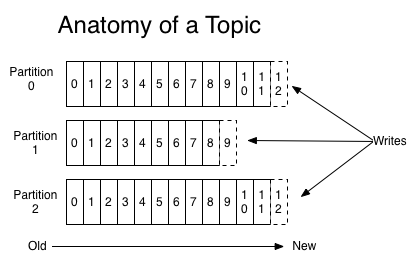
\includegraphics[width=0.7\linewidth]{Figures/log_anatomy}
    \caption[How partition works in a kafka topic]{How partitioning works in a kafka topic. Source: \cite{kafka_doc}}
    \label{fig:loganatomy}
\end{figure}

Only the offset or position of a consumer is retained as metadata, on a per-consumer basis. This offset is completely controllable by the consumer, so that if normally it would advance linearly, the consumer could consume records in any possible order. For example, a consumer can reset to an older offset or, conversely, skip ahead to consume data from the latest record, according to its own policy.

The partitions in the log allow for scaling beyond a size that could fit on a single server, since a topic can handle an arbitrary amount of data, but each individual partition must fit on the servers that host it, and act as the unit of parallelism, so that it's possible to increase the number of partitions of a topic as needed, according to the required throughput.

\subsection{Producers and Consumers}

\paragraph{Producers} They are the components that publish the data to the topics of their choice. They handle the assignment of each record to the partitions within the topic. This is usually done according to a round-robin scheduling, to favour balance loading, or otherwise with a semantic partition function (e.g. the key of a record).

\paragraph{Consumers} They are labelled with a \textit{consumer group} name, and each record published to a topic is consumed by one consuming instance within each subscribing consumer group. Each instance can be in separate processes or even on separate machines.

A common configuration has topics with a small number of consumer groups, one for each "logical subscriber", where each group, for scalability and fault tolerance purposes, is composed of many consumer instances.

\begin{figure}[h]
    \centering
    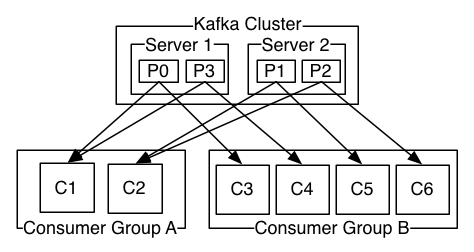
\includegraphics[width=0.7\linewidth]{Figures/consumer-groups}
    \caption[Consumer groups subscribing to a Kafka Cluster]{Consumer groups subscribing to a Kafka Cluster. Source: \cite{kafka_doc}}
    \label{fig:consumer-groups}
\end{figure}


The way Kafka implements consumption is by dividing up the partitions in the log over the consumer instances so that each instance gets a "fair share" of partitions reserved at any point in time. If new instances join the group, Kafka will handle dynamically this addition by giving away some partitions from other members of the group, in order to preserve the fair sharing. Otherwise, if an instance dies, its partitions will be distributed to the remaining instances.

A total order over records is provided only within a partition, and not between different partitions in a topic. However, if a total order over records within a topic is required, than a single partition is needed, consequently meaning that there can only be one consumer process per consumer group. 

\subsection{Use cases}

\paragraph{Messaging}

Kafka can be used as a replacement for a more traditional message broker, for reasons such as decoupling processing from data producers and buffering unprocessed messages. In comparison to most messaging systems, Kafka provides replication, better throughput, built-in partitioning and fault-tolerance, being then a very good solution for large scale message processing applications.

In this domain, Kafka can be compared to  \href{https://www.rabbitmq.com/}{RabbitMQ} and \href{http://activemq.apache.org/}{ActiveMQ}, two of most used traditional messaging systems.

\paragraph{Log Aggregation}

Log aggregation usually collects log files off servers and puts them in a central place, such as a file server or HDFS, for processing purposes. Kafka gives a cleaner abstraction of log or event data as a stream of messages, abstracting away the details of files and allowing, in addition, for lower-latency processing and easier support for multiple data sources and distributed data consumption. In comparison to log-centric systems like Flume, Kafka offers a much lower end-to-end latency and stronger durability guarantees due to replication, while providing equally good performances. 
 
\paragraph{Activity Tracking \& Metrics}

The original use case for Kafka was to rebuild a user activity tracking pipeline as a set of real time publish-subscribe feeds. Thus decomposing site activity, such as page views, searches, or other actions users may take, publishing records to one topic per activity type. These feeds would be available to subscription for real time processing or monitoring, and loading into any data warehousing system for offline processing and reporting.

Kafka is often used for aggregating statistics from distributed applications in order to produce centralized feeds for operational monitoring purposes, providing a fault-tolerant monitoring pipeline with low latency.


\section{NiFi}

\textbf{Apache NiFi} \cite{nifi_doc} is a distributed system for centralising, processing and distributing streams of data across a cluster. Its most notable feature is a web GUI allowing to visually structure the data flow directly from the sources through the definition of graphs where each vertex is called \textbf{Processor} and each edge in-between is a queue in which the \textbf{Flowfiles}, objects wrapping a single records, wait if the processor is busy.

NiFi allows for the creation of a secure cluster where each node takes care of processing a fraction of the Flowfiles circulating inside the graph, load balancing in case of node failures. 

\subsection{FlowFiles}

A \textbf{FlowFile} represents a single piece of data in NiFi, made up of two components: \textbf{FlowFile Attributes} and \textbf{FlowFile Content}. The FlowFile Content is the actual payload, the data that is represented by the FlowFile, while the attributes are characteristics that provide information or context about that data, consisting of key-value pairs. 

All FlowFiles have the following standard attributes:

\begin{itemize}
    \item \textbf{uuid}: A unique identifier for the FlowFile
    
    \item \textbf{filename}: A human-readable filename that may be used when storing the data to disk or in an external service
    
    \item \textbf{path}: A hierarchically structured value that can be used when storing data to disk or an external service so that the data is not stored in a single directory, that is its location on the system
\end{itemize}

\subsection{Processors}

As already mentioned a \textbf{Processor} is the basic block for the graph structure of a NiFi flow. There are a great variety of Processors built in, ranging in function from database connections for insertions or queries to producers and consumers for queue processes such as Kafka; from object manipulation such as JSON or XML splitting and fetching to ingestion from sources like web sockets or filesystems.

A single processor can be scheduled to run periodically or continuously and can be configured with the number of concurrent threads that can be used for the execution. Each Processor has different output ports according to the results of the Flowfile processing: \textit{success}, \textit{failure} or other processor-specific routes (e.g. \textit{\textbf{SplitText}} processor, used to split text according to user-specified rules has \textit{original} and \textit{splits} as additional output ports, used to convey in different routes Flowfiles both before and after being split).
\chapter{Data Processing}

Data Processing is the layer immediately following the Data Quality: once data have been formatted and cleansed, adapted then to our needs, we can start analysing and processing them through the use of adequate frameworks, in order to extract from, transform and enrich them for visualization purposes.\\

\section{Data Processing Techniques}

\subsection{Batch Processing} \label{BatchProc}

Batch data processing is the most classical data processing mode and is characterised by the delayed execution and the simultaneous processing of data in chunks (batches) loaded from a dataset.
\\
\newline
The processing is divided in three phases, at first data are collected for an extended period of time, after that period the batch of collected data is loaded to the processing component where it is modified concurrently as a whole, with transformation like Map and Reduce; finally the processed batch is written again on the database.
\newline
\\
The main advantages of this method are that it efficiently processes high volumes of data and transactions, and that processing can be scheduled at fixed times or when the machines' load is light; the main drawback is that it is not suited for real time applications which are becoming more and more prominent.

\subsection{Graph Processing} \label{GraphProc}

A graph in data science is a representation of entities and their relationships.\newline
Entities are represented as nodes, the vertices, and the relationships as edges between those nodes.\newline
\\
Data represented in such way is useful to represent information where connection is as important as the entity, such as people's friends networks or the world wide web; and requires a very different processing model in respect to other structured data.\newline
\\
A widely used Graph processing system is Apache Giraph used for Facebook friends' networks, which implements the architecture described in Google's project Pregel paper for large-scale graph computing\cite{Malewicz:2010:PSL:1807167.1807184}.
\\
Both Apache Spark and Flink feature plugins for the support of graph analytics.

\subsection{Stream Processing} \label{StreamProc}

Streaming data processing differentiates itself from the classic data processing for its use of unbounded datasets, that is a continuous and endless data flow which needs adequate abstractions in order to be able to apply operators or transformations like Map, Reduce and Filter operations. \\ 

Generally, there are 2 execution models usable when to approach an unbounded dataset:

\begin{itemize}
    \item \textbf{Streaming}: continuous elaboration as long as data are being produced.
    \item \textbf{(Micro-)Batch}: finite time execution, which releases resources when the batch processing ends.
\end{itemize}

A Batch based execution is feasible when requirements on the state management, in-order consuming and windowing are not present or very relaxed and, thus, a Streaming approach is generally favoured because of the conceptual paradigm which defines it: Dataflow Programming.

\paragraph{Dataflow Programming}  \label{DataflowProg}

Dataflow Programming is a programming paradigm which models an application as a Direct Acyclic Graph (DAG) and thus it differentiates itself very heavily from the Imperative Programming (or Control Flow), which models a program like finite sequence of operations.\\
This paradigm emphasizes the continuous flow of data between operators, defined as Black Boxes with explicit input and output ports used to connect with other operators. An operation runs as soon as all of its inputs become valid. Thus, dataflow languages are inherently parallel and can work well in large, decentralized systems \cite{Johnston:2004:ADP:1013208.1013209}.

\pagebreak

\section{MapReduce} \label{MapReduce}

\textbf{MapReduce} \cite{hadoop_doc} is a framework, part of Apache Hadoop, named after its algorithm, engined to be run on YARN to deploy applications able to process data in batches from HDFS or distributed databases. \\

\subsection{Structure}
The framework's management is handled by two tracker components, the \textbf{Job Tracker} who acts as a master and the \textbf{Task Trackers} who run on the single nodes, act as slaves and carry out the tasks issued by the \textbf{Job Tracker}.

The \textbf{Job Tracker} manages available resource and the MapReduce job's lifecycle.\\ It is responsible for the load distribution using a Data Locality policy, so that nodes are chosen to process data present in their file system if possible or at least from a machine in the same rack. This way the overhead caused by the sending of data is minimised.
\\
The \textbf{Job Tracker} is also responsible for the framework fault tolerance, checks the liveness of tasks and nodes and reschedules failed tasks.

\subsection{Process Flow}

A MapReduce job usually involves six steps:

\begin{enumerate}
	\item \textbf{Load dividing}: The framework elects some nodes to load the Map function and some others to load the Reduction function.
	\item \textbf{Input handling}: The framework divides the whole data set in batches and formats the input to the appropriate key, value pair; each batch is sent to a node marked with a Map for processing.
	\item \textbf{Mapping}: Each Map node applies the Map function defined by the developer to the list of key, value pair in its batch and outputs a transformed list of key, value pairs
	\item \textbf{Shuffling}: The framework sorts and shuffles the pairs output by the Mapping so that pairs with the same key are sent to the same Reduce node.
	\item \textbf{Reducing}: Each Reduce node applies the Reduce function defined by the developer to the Mapped list of key, value pair and for each key aggregates all values and produces one or more transformed pairs.
	\item \textbf{Output handling}: The framework collects all outputs from Reduce nodes and writes it onto HDFS or a DB, usually the same whence the input data set came
\end{enumerate}

 \pagebreak
 
\section{Spark} \label{Spark}

\href{https://spark.apache.org/}{\textbf{Apache Spark}} \cite{spark_doc} is an open source distributed computational framework originally developed at Berkeley and now maintained by the Apache Software Foundation.
\\
Conceived as a general multiplatform engine, Spark can run as standalone, on YARN or on Apache Mesos; can access data from standard File Systems, from HDFS or any distributed database and can be used for Batch Processing, Graph Processing (thanks to GraphX plugin) or Stream Processing.
\\
\\
The problem that sparked its creation was MapReduce's inefficiency in applications that use the same working set of data on multiple parallel operations, among which are included: iterative machine learning algorithms and interactive data analysis tools \cite{Zaharia:2010:SCC:1863103.1863113}; Spark's aim is to support such applications while providing scalability and fault tolerance.
\\
In order to do that, Spark uses a typical architecture with a \textbf{Driver Program} that runs the developer application's main() and executes parallel task on the clusters and its main abstraction: Resilient Distributed Dataset (RDD).

\subsection{Resilient Distributed Dataset}
RDD is a collection of elements partitioned across the cluster's nodes in a fault tolerant way that can be processed in parallel, persisted in memory to be used iteratively and efficiently by parallel operations; an RDD is usually instantiated from an input file loaded from HDFS or a distributed database; operations are then processed on it through classical Map, Filter and Reduce functions, a series of these operations will produce a graph with the execution planned called \textbf{lineage}, from the \textbf{lineage} an RDD can be reinstated to its proper state even after failure.
Beside these features RDD also has the following traits:
\begin{itemize}
	\item In-Memory, data inside RDD is stored for as long and as much as possible in memory (RAM), as opposed to the disk-oriented methods of MapReduce.
	\item Immutable, RDDs do not change once created, and can only be transformed through the instantiation of a new RDD.
	\item Lazily evaluated, data inside RDD is not available nor transformed until an action is executed that requires access to those data.
	\item Cacheable, data can be held in a persistent storage like memory or, worse comes to worst, disk.
	\item Parallel, RDD process data in parallel.
	\item Typed, RDD records have types such as Int or String.
	\item Partitioned, records are partitioned and distributed across several nodes.
\end{itemize}

\subsection{Extensions}
\subsubsection{GraphX}

GraphX is an extension of Spark for graphs and graph analysis. GraphX extends RDD adding a Graph abstraction implemented as a directed multigraph with properties attached to both vertices and edges and exposes typical graph operators, while also providing an optimized variant of the Pregel API.

\paragraph{Property Graph}

The Graph abstraction, or property graph is a directed multigraph with properties attached to each vertex and edge defined by the developer. A directed multigraph is defined as a directed graph where more than one edge can connect two nodes, as two nodes might have multiple relationships with different properties, (i.e. Annie and Barb are both colleagues and friends). \\ \\
Property graphs, like RDDs, are immutable and to transform them a new one must be instantiated from the former through an operation, they are distributed across executors using vertex partitioning heuristics and are fault-tolerant thanks to the same lineage mechanism seen in RDDs.

\paragraph{Graph Operations}

Graphs implement several operators that can be divided in three classes

\begin{itemize}
	\item Property Operators: The Graph equivalent to RDD map, with the difference that you can choose to run map over the vertices, the edges, or the <source node, edge, destination node> triplets , to modify the properties of said components.
	\item Structural Operators: Which act on the topology of the graph, an example would be reverse which, from a Graph, returns a new Graph where all edges' directions are reversed.
	\item Join Operators: Used to join properties from different graphs or from external collections like RDDs.
\end{itemize}


\subsubsection{SparkStreaming}

SparkStreaming in an extension of Spark developed to enable live data stream processing in the falut-tolerant and highly scalable framework provided by Spark while maintaining a high throughput.
The ingested stream source can be any major Apache source like Kafka, Flume and Nifi; other streams like Amazon Kinesis, File Systems like HDFS or S3 and TCP sockets.
The stream can be processed through the high-level functions like map, reduce and join and finally output to File System and Distributed Databases.

\paragraph{DStream}

DStream, short for Discretized Stream, is the main abstraction introduced by SparkStreaming, which represents a continuous stream of data. \\
As for RDDs, DStreams can be instantiated from a stream source like Kafka, Flume and Kinesis, or by applying a transformation on another DStream like map. As it stands DStreams are in fact sequences of RDDs, maintaining therefore their properties of being Distributed and Fault-Tolerant.
\\ \\
Internally a continuous stream of data, splits the live flow into mini batches which are then sent to the Spark Engine that can then process them as batches and output them to processed batches as previously seen.

\subsubsection{MLlib}

Machine Learning Library, or MLlib for short is a set of APIs for Spark that expose several tools for Machine Learning using Spark as a backend taking advantage of Spark's efficiency in iterative algorithms.

MLlib exposes a selection of Machine Learning algorithms for classification, regression, creation of decision trees and random forest, recommendation, clustering, topic modelling and pattern mining.
It also offers other tools to transform features, to handle datasets and hyperparameters and to make computation with distributed linear algebra and statistics.

\pagebreak
\section{Flink}\label{Flink}

\href{https://flink.apache.org/}{\textbf{Apache Flink}} \cite{flink_doc} is an open source framework developed for the continuous and distributed processing of data flows. Based on the Dataflow Programming model, it provides a set of abstractions specifically designed for real time stream processing.

\subsection{Abstraction levels}  \label{AbstractionLevels}

\begin{itemize}
	\item \textbf{Stateful Streaming}: It's the lowest abstraction layer, which allows developers to freely manage data flows and their processing, use fault-tolerant states and callback registration on events.
	\item \textbf{Core API}: it's the basic API, which is divided between \textbf{DataStream API}, specifically conceived for bounded and unbounded dataset processing, and \textbf{DataSet API}, implemented as a special case of the first API set, used only for bounded datasets. These 2 APIs offer transformations and operations like unions, aggregations, windowing and state management, needed for the data flow upon which they are applied.
	\item \textbf{Table API}: it's a declarative DSL \footnote{Domain Specific Language: a language with a limited expressiveness which focuses on a given domain of use.} which follows the extended relational model and offers the possibility to model a data stream like a table upon which it's possible to execute operations like projections, aggregations and groupings. Despite being less expressive with respect to the Core API, they allow for a greater compactness when it comes to describing the operations to be executed on the data.
	\item \textbf{SQL}: it's the highest level of abstraction offered by Flink and interacts directly with the Table APIs in order to provide a representation of the application being developed through SQL queries. It can be executed on the tables defined by the Table API, directly on the data.
\end{itemize}

\subsection{Programs Dataflows}  \label{ProgramsDataflows}

The base elements of a Flink application are the following:

\begin{itemize}
	\item \textbf{Streams}, data structures containing data.
	\item \textbf{Transformation Operators}, which can change the stream, for example, via aggregations, groupings, mappings and reductions.
	\item \textbf{Sources}, they are primary data entry points and can be files or records from queues like Kafka. They are the starting nodes of the application DAG.
    \item \textbf{Sinks}, They are the application output, being it a file, any process or another queue. They are the ending nodes of the application DAG.
\end{itemize}

\begin{code}

\begin{minted}[breaklines]{Scala}
val lines = env.addSource(new Consumer[String](...))

val events = lines.map(line -> parse(line))

val stats = events
            .keyBy("id") // Stream is partitioned by the key "id" 
            .timeWindow(Time.seconds(10)) // All the events in the given window are considered 
            .apply(MyWindowAggregationFunction()) // All the records are aggregated according to the function      

stats.addSink(new RollingSink(path))
\end{minted}

\end{code}

\begin{figure}[h]
	\centering
	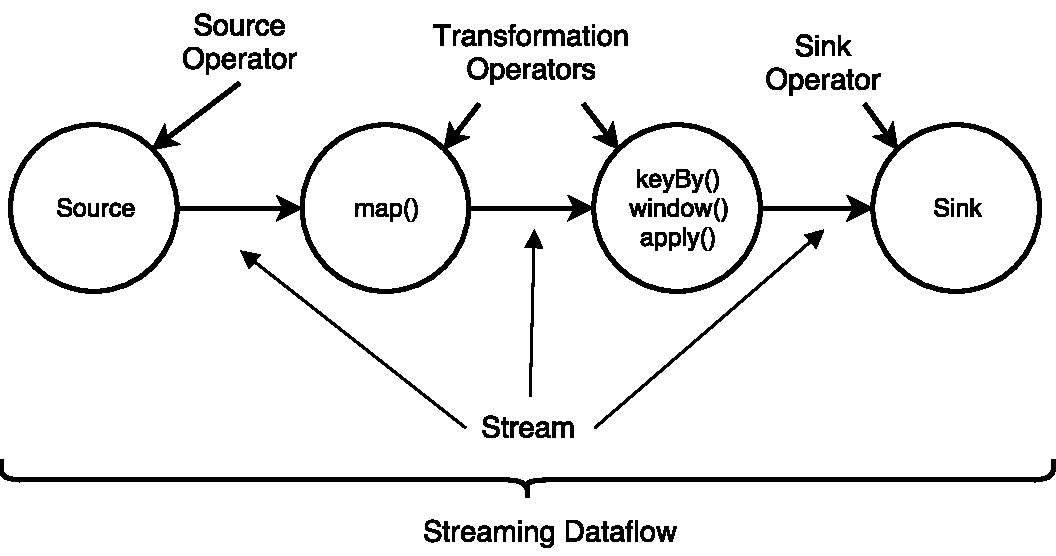
\includegraphics[scale=0.75]{Figures/dataflow.pdf}
	\decoRule
	\caption[Streaming Dataflow]{DAG outlining the previous code snippet}
	\label{fig:Dataflow}
\end{figure}

\paragraph{Event Time}

Flink supports different notions of time in streaming programs \cite{flink_eventtime} and each of them can be useful for specific use cases:

\begin{itemize}
    \item \textbf{Processing time} refers to the system time of the machine that is executing the respective operation.
    
    When it is being used, the system clock of the machines will be used to run all time-based operations. Being the simplest notion of time, no coordination between streams and machines is required, providing, this way, the best performance with the lowest latency. However, since the entire environment is distributed and can work asynchronously, processing time does not provide determinism, because of its susceptibility to the speed at which records arrive in the system and flow between each pair of operator inside the system.
    
    \item \textbf{Event time} is the time embedded within a record, representing when it occurred on its producing device. This time is typically assigned before records enter Flink and it can be extracted directly from the record. An event time window of an hour will contain only records carrying an event timestamp within that hour, regardless of their actual time and order of arrival.
    
    Event time is especially useful when dealing with out-of-order or late events, and even on replays of data from persistent logs or backups. When using event time, the progress of time is discretized based on the data, rather than the clock and, for this reason, the generation of the Event Time Watermarks, central to the mechanism that signals progress in event time,  must be specified internally to the program.
    
    Event time processing causes inherently a certain latency, due to its waiting for late and out-of-order events.
    
    \item \textbf{Ingestion time} is the time that events enter Flink. The source operator assigns to each record its current time as a timestamp, which all time-based operations refer to.
    
    Ingestion time can be considered an alternative sitting, conceptually speaking, in between event time and processing time: it is more expensive than processing time, while providing deterministic results, as it uses stable timestamps, assigned once at the source, used by all of the following time-based operations, but cannot handle any out-of-order events or late data, with respect to event time, even though there's no need to specify the watermarks generation.
\end{itemize}


\paragraph{Windows}

Windows are the core mechanism within a stream processing framework. They allow the application of operations after splitting the stream into \textit{buckets} of finite size. The structure of a windowed Flink program differs when considering \textbf{keyed} and \textbf{non-keyed} streams: a keyed stream is split into multiple logical sub-streams and a window is applied to each one of them separately, differently from a non-keyed stream where the window is applied globally and within a single task \cite{flink_windows}.

A Window lifecycle starts as soon as the first element belonging to it arrives and ends, being completely removed, when the time, event or processing time, passes its end timestamp plus any user-specified \textbf{allowed lateness}. For example, in an event-time-based Flink application where a tumbling window is created every 5 minutes with an allowed lateness of 1 minute, a new window will be created for the interval between 11:30 and 11:35, as soon as a record with a timestamp falling into that interval arrives, and will be removed when the watermark passes the 11:36 timestamp.

For each window must be specified a \textbf{Trigger} and a function (\texttt{WindowFunction}, \texttt{ReduceFunction} or \texttt{FoldFunction}) attached to it: the Trigger is used to specify the conditions under which the window is considered ready or complete for the function to be applied, while the function will contain the operation to be applied to the contents of the window. The triggering policy is completely customizable and can even decide to purge a window’s contents, leaving the window metadata untouched, in order to add new data to that window.

It's possible specify an \textbf{Evictor}, used to remove elements from the window after the trigger fires and before and/or after the function is applied.

There are four main window assigners usable in Flink:

\begin{itemize}
    \item \textbf{Tumbling Windows} are fixed size and non-overlapping windows, which are configured with a parameter controlling how much frequently a new window has to be started.
    \item \textbf{Sliding Windows} are fixed size, similarly to tumbling windows, but are configured with an additional slide parameter, which controls how frequently a sliding window is started. Therefore they overlap and elements are assigned to multiple windows.
    \item \textbf{Session Windows} group elements by sessions of activity. Session windows do not overlap and do not have a fixed start and end time, in contrast to tumbling windows and sliding windows. A session window closes when it does not receive elements for a certain period of time, i.e., when a gap of inactivity occurred.
    \item \textbf{Global Windows} assign all elements with the same key to the same single global window. This windowing scheme is only useful if you also specify a custom trigger. 
\end{itemize}



\paragraph{Parallelism} \label{ParallelismFlink}

Applications using Flink are inherently parallels and distributed. During execution, a stream may be divided in more than one partition; each operator can have more than a single sub-task operating on data, each one independent from the other and executed on different threads or, if possible, on different machines or containers.\\
The parallelism of a task is the parameter indicating the number of subtasks an operator can have and, consequentially, the number of partitions of the stream getting outputted from that operator.\\

\begin{figure}[!htb]
    \centering
    
\includegraphics[scale=0.75, trim=0.5cm 12cm 1cm 0.5cm]{Figures/parallel_dataflow.pdf}
    \decoRule
    \caption[Parallel Dataflow]{DAG with Parallelism=2}
    \label{fig:ParallelDataflow}
\end{figure}

Streams can transport data between a pair of operators following two different patterns: One-to-one pattern and redistributing pattern:
\begin{itemize}
	\item \textbf{One-to-one streams} preserve the stream partitioning and the order of the elements passed to the following operator. For example, the subtask[0] of a map() operator will get to see the same elements produced by the subtask[0] of the previous Source operator.
   
    \item \textbf{Redistributing streams} change their partitioning, sending the data to different subtasks, based on the transformation being applied. For example, a keyBy() operator repartitions the stream using the hash of the chosen key. In this case, the elements' order will be preserved only between neighbouring operations pairs, and won't be ever guaranteed being the same in the following operators.
\end{itemize}

\subsection{Data Streaming Fault Tolerance}

Flink offers built-in guarantees in case of failures, so that there's minimum disruption on the processing jobs and a consistent recovery of the data streaming applications' state. The two main features which allows recovery from errors or runtime exceptions are \textbf{Checkpoints} and \textbf{Savepoints}.

In case of a program failure (due to machine-, network-, or software failure), Flink stops the distributed streaming dataflow, restarting the operators and resetting them to the latest successful checkpoint, while also resetting the input streams to that same point of the state snapshot. Any records processed as part of the restarted parallel dataflow are guaranteed to not have been part of the previously checkpointed state.

For this mechanism to realize its full guarantees, the data stream source, being it a message queue or a broker, needs to be able to rewind the stream to a defined recent point. Apache Kafka, thanks to its offsets, has this ability and Flink’s connector to Kafka makes use of that ability.

\subsubsection{Checkpoints}

\begin{code}
    \label{code:checkpointing}
    \begin{minted}[breaklines, breakbefore=., breakafter=(]{Scala}
    val env: StreamExecutionEnvironment = StreamExecutionEnvironment.getExecutionEnvironment
    
    env.enableCheckpointing(60000)
    
    env.getCheckpointConfig.enableExternalizedCheckpoints(ExternalizedCheckpointCleanup.RETAIN_ON_CANCELLATION)
    
    env.setStateBackend(new FsStateBackend(state_dir, true)) 
    \end{minted}
    \captionof{listing}{An example of asynchronous checkpointing configuration on a FileSystem backend}
\end{code}~\\

\textbf{Checkpoints} are Flink's tool to guarantee automatic fault tolerance and recovery of the job's state, in case of runtime errors or failures \cite{flink_checkpointing}. 
\\
\\
They are, essentially, snapshots of the current state of the job that act consistently as the system fall back in case of failure. Flink’s mechanism for drawing these snapshots is inspired by the standard Chandy-Lamport algorithm \cite{Chandy:1985:DSD:214451.214456} for distributed snapshots and is specifically tailored to Flink’s execution model \cite{DBLP:journals/corr/CarboneFEHT15}. 
\\
\\
Checkpointing must be configured on the application level as shown in the previous snippet by calling the \texttt{enableCheckpointing(milliseconds)} to specify how much time should pass between two consecutive snapshots. By default, if a job is cancelled the checkpoint is deleted as well, so the retainment on cancellation must be enabled manually. 
\\
\\
An additional configuration available to application level setup is the State Back-end, that is the location where the checkpoint, thus, the job's state, should be saved. There are three possible back-ends which can be chosen from: \textbf{in Memory}, useful for testing, on a \textbf{Filesystem} (local or distributed, like HDFS) and on \textbf{RocksDB}\footnote{\href{http://rocksdb.org/}{RocksDB} is an embeddable persistent key-value store for fast storage}, particularly recommended for huge states. Optionally, snapshots can be taken asynchronously in order not to block the processing pipeline.
Checkpoints can be used to manually recover from failures through specific commands from Flink CLI, but they don't support scaling on recovery, that is, parallelism can't be changed when recovering from a snapshot.

\paragraph{Barriers}

A core element in Flink’s distributed checkpointing are the \textit{stream barriers}: lightweight elements flowing with the records, as part of the data stream, injected into the stream starting from the data source, without interrupting it. They are used to separate the records in the data stream belonging to two consecutive snapshots. Each barrier contains the ID of the snapshot whose records were pushed in front of it: there can be multiple barriers belonging to different snapshots, meaning that checkpoints may happen concurrently.
\\
\begin{figure}[!htb]
    \centering
    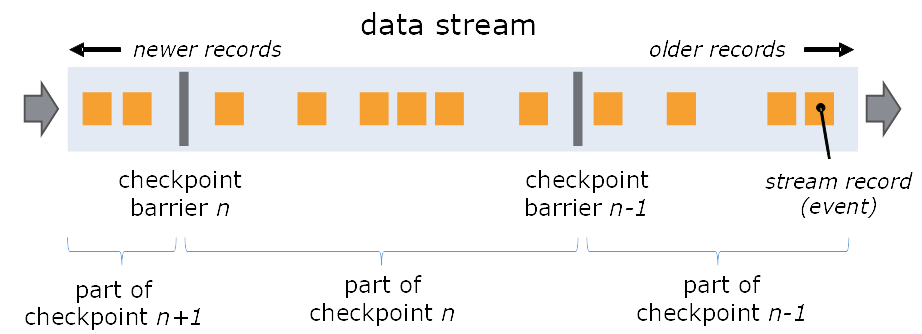
\includegraphics[width=1\linewidth]{Figures/stream_barriers}
    \caption{Visual representation of Stream Barriers}
    \label{fig:streambarriers}
\end{figure}
\\
Let's call $S_n$ the point in the stream where the barriers for snapshot $n$ are injected, representing the position up to which the snapshot covers the data, reported to the checkpoint coordinator, Flink’s JobManager.
\\\\
Flowing downstream, each intermediate operator must receive a barrier for snapshot $n$ from all of its input streams before, then, emitting a barrier for the same snapshot into all of its outgoing streams, until a sink operator is reached. Once a sink has received a barrier $n$, from all of its input streams, the snapshot $n$ is acknowledged to the checkpoint coordinator and the checkpoint is considered complete.

At the completion of snapshot $n$, the job will never ask the sources to replay the records from before $S_n$, since they all went through the topology.
\\\\

If an operator receives more than one input stream, an \textit{\textbf{alignment}} step must be performed between all of the inputs:

\begin{itemize}
\item As soon as the operator has received a snapshot barrier $n$ from an incoming stream, it must wait the same barrier from all of the other inputs, since otherwise processing would mix records belonging to consecutive snapshots and, in this case, would use also the barriers for snapshot $n+1$.

\item While waiting, all barriers $n$ are temporarily set aside and the corresponding records put in an input buffer.
    
\item Once the last stream has received barrier $n$, the operator emits all pending outgoing records and then snapshot $n$ barriers itself, before continuing processing records, starting from input buffers and then the actual input streams.
\end{itemize}

\paragraph{Exactly Once vs. At Least Once}

The alignment step previously described may add latency to the streaming program, usually negligible, being in the the order of a few milliseconds, but some applications' latency may increase noticeably. If consistent super low latency (few milliseconds) for all records is a strict requirement, Flink allows to skip the stream alignment during a checkpoint, but snapshots are still drawn as soon as an operator has seen the checkpoint barrier from each input stream.

As a consequence, the operator keeps processing all inputs, including elements belonging to checkpoint $n+1$, which will then occur as duplicates when restoring the state of the stream because they are both included in the state snapshot of checkpoint $n$ and part of the data following this same checkpoint.
\\

The alignment step happens only when operators with multiple predecessors (join operators) or 
multiple senders (such as a stream repartitioning/shuffle) are present. For this reason, dataflows containing only parallel streaming operations (\texttt{map()}, \texttt{flatMap()}, \texttt{filter()}, …) guarantee \textit{exactly once} semantics even in \textit{at least once} mode.

\subsubsection{Savepoints}

\begin{code}
    \label{code:savepoint}
    \begin{minted}{Bash}
flink savepoint <jobId> [<savepointDirectory>] -yid <yarnAppId> 
    \end{minted}
    \captionof{listing}{Savepoint triggering from the Flink CLI}
\end{code}~\\

\textbf{Savepoints}, just like checkpoints, serve the purpose to save the state of a Flink application in case of cancellation or failures. Differently from checkpoints, they can only be performed manually from Flink CLI, but support parallelism rescaling and they're the go-to choice when Flink's application computational capabilities must be improved by setting an higher parallelism factor or when an upgrade to a more recent version of Flink must be performed. Savepoint's mechanism works such that it associates each application's stateful operator, to its own state in a map-like structure: for this very reason, in order to successfully preserve state when upgrading a Flink application, each stateful operator needs to have its own \texttt{uid} set.

\subsection{High Availability}

A Flink's setup, whether a standalone cluster (being it containerized or physical) or using Distributed Resource Managers such as \nameref{YARN} or Mesos\footnote{\href{https://mesos.apache.org/}{Mesos} is a distributed cluster manager used to manage datacenters with a master-slave architecture. It's a lower level abstraction with respect to YARN and thus performs a different job more inclined towards machines management and task scheduling, than purely job's scheduling.}, is made of a Job Manager and one or more Task Managers, each one with one or more parallelism slots (cores usable for processing). Task Managers (TMs) handle jobs actual executions, while the Job Manager (JM) handles TM orchestration and monitoring and, for this reason, is a single point of failure, whose crash causes the entire Flink cluster to stop.
follows the principles of a Active-Standby architecture (also used by HDFS Namenode e YARN Resource Manager HA set-ups) where a single leading JM is active, while multiple JMs standby, ready to take over leadership in case the leader failure. This guarantees that there is no single point of failure and programs can make progress as soon as a standby JM has taken leadership. There is no explicit distinction between standby and master JM instances: all of the possible JMs are registered as masters to \textbf{Zookeeper}, which is going to handle failure scenarios.

In case of YARN clusters configured in High Availability mode, a single JM, being the \textbf{Application Master}, is still run, but YARN itself will restart its container on failures. As additional configuration, the maximum number of attempts for the application masters needs to be configured in the YARN configuration.

\subsection{Flink Extensions} \label{FlinkLibs}

\subsubsection{FlinkCEP: Complex Events Processing}

FlinkCEP is a Flink extension adding the possibility to analyse events pattern in a DataStream, thanks to the Pattern API. This API allows the definition of patterns to be found in a stream and their selection in order to create a new DataStream of Alerts.\\


\begin{code}
\label{code:pattern-example}
\begin{minted}[breaklines]{Scala}

val inputStream: DataStream[SensorEvent] = ...

val pattern = Pattern.begin("start").where(_.getId == 42)
.next("middle").subtype(classOf[TemperatureEvent]).where(_.getTemperature >= 90.0)
.followedBy("end").where(_.getName == "end")

val patternStream = CEP.pattern(inputStream, pattern)

val result: DataStream[Alert] = patternStream.select(createAlert(_))
\end{minted}
\captionof{listing}{An example of Pattern API usage}
\end{code}~\\

In FlinkCEP, a \textbf{Pattern}, similarly to a pattern of a Regular Expression, can be \textbf{single} or \textbf{iterative}. For example, in a pattern like \texttt{"a b+ c? d"}, \texttt{a}, \texttt{c?} e \texttt{d} are single patterns, while \texttt{b+} is iterative.
\\

In a Pattern there can be, analogously to Regular Expressions, Quantifiers and Conditions.

\paragraph{Quantifiers}

Iterative patterns can be specified with the following self explanatory methods:

\begin{itemize}
    \item \texttt{pattern.oneOrMore()};
    \item \texttt{pattern.times(\#ofTimes)};
    \item \texttt{pattern.optional()}
\end{itemize}

\paragraph{Conditions}

Each pattern can have additional conditions specified, which can be related to a property of an incoming event, or the contiguity to other events.

Methods \texttt{pattern.where()} and \texttt{pattern.or()} can be used to specify \texttt{\justify{IterativeCondition}}s, \texttt{SimpleCondition}s or a combination of multiple conditions. In this case, combinations can be specified concatenating all the previous methods, including the quantifiers, optionally adding more constraints on the contiguity of the same pattern by calling \texttt{consecutive()}, for the strict contiguity, and \texttt{allowCombinations()} for the relaxed non-deterministic contiguity.
\\
Some examples:

\begin{code}
\label{code:iterative-cond}
\begin{minted}[breaklines]{Scala}
middle.oneOrMore().where(
    (value, ctx) => {
        lazy val sum = ctx.getEventsForPattern("middle")
                          .asScala.map(_.getPrice).sum
        value.getName.startsWith("foo") && sum + value.getPrice < 5.0
    }
)
\end{minted}
\captionof{listing}{Iterative Condition}
\end{code}~\\

\begin{code}
    \label{code:simple-cond}
    \begin{minted}[breaklines]{Scala}
//Example of conjunction through where concatenation
start.where(event => event getName startsWith "foo" ) )
     .where(event => event getTotal equals 50  )

start.subtype(classOf[SubEvent]).where(subEvent => ... /* some condition */)
    \end{minted}
    \captionof{listing}{Conditions combinations}
\end{code}~\\

\paragraph{Pattern Combination}

Similarly to conditions combination, pattern combination is possible through the consecutive calls to the following methods allowing to specify the contiguity constraints which a given pattern should satisfy:

\begin{itemize}
    
    \item \texttt{next()}, for strict contiguity.
    \item \texttt{followedBy()}, for relaxed contiguity.
    \item \texttt{followedByAny()}, for non deterministic relaxed contiguity.
    \item \texttt{notNext()}, NOT pattern with strict contiguity.
    \item \texttt{notFollowedBy()}, NOT pattern with relaxed contiguity.

\end{itemize}

Each pattern combination can be followed by a time constraint specified by concatenating \texttt{within(Time)}.

\paragraph{Pattern Detection}

Once a pattern sequence has been specified, it needs to applied to the target \texttt{Datastream}, creating this way a \texttt{PatternStream}.
On this new stream \texttt{select} or \texttt{flatSelect} operations need to be applied in order to enable further processing on the events satisfying the pattern.

\subsubsection{Other extensions: Flink Gelly and FlinkML}

In addition to the aforementioned library for complex event handling, Flink makes specific sets of API available, which provide useful tools when it comes to enable advanced processing on data.

\paragraph{Flink Gelly} is an API based on the Flink \texttt{Dataset}s API specifically developed for Graph Processing. Graphs are stored as a finite set of vertices and edges, a special case of a \texttt{Dataset}. This library allows the application of operators like Map, Filter, Intersect and Union, Mutations like edge and vertex removal, but also advanced techniques belonging to Graph Theory like \textit{Iterative Graph Processing} (Vertex-centric, Scatter-Gather and Gather-Sum-Apply), \textit{Single Source Shortest Paths}, \textit{Clustering} and Similarity analysis.

\paragraph{FlinkML} is a set of tools which allows the application of Machine Learning techniques on Flink data streams, including both algorithmic implementations for supervised (\textit{SVMs} and \textit{Multiple Linear Regressors}) and unsupervised (\textit{K-nearest neighbours}) learning, Data Preprocessing and Recommendation (\textit{ALS}).



\chapter{Data Visualization}

Data Visualization is the visual representation of data using plots and visual models. In the infrastructural stack stands at the highest level since it's the mean through which the result of all the processing is shown. The reason that makes it so important is that humans are not able to extract useful information from raw data at a glance, and thus comes the need for clear and intuitive plots capturing all the helpful statistics contained, in a concise way: insights from which human can act accordingly.

The stack uses as a visualization tool Tableau, and in this chapter will be presented its structure and its strengths. 

\section{Introduction}

Tableau is a software dedicated to creation of visualizations for the Business Intelligence. According to Gartner \cite{gartner_tableau}, Tableau offers an highly intuitive and interactive way to the access, manipulation and analysis of data, without the need for coding, positioning itself among the first three product leaders in the sector. Tableau's main features include easiness and intuitiveness in the software use, data sources management and some innovative features such as table calculations and the possibility to use data analysis techniques directly on the plots.

Tableau On Premise version is composed of two elements:

\begin{itemize}
    \item \textbf{Tableau Desktop}: Allows for the creation of worksheets, dashboards and stories, linked to one or more data sources.
    \item \textbf{Tableau Server}: It is used to publish the plots created with Tableau Desktop, in order to make them available to end users.
\end{itemize}

\section{Tableau Desktop}

Tableau is structured in a Microsoft Excel fashion, with workbooks and sheets: a workbook is made of many sheets which can be worksheets, dashboards or stories. A worksheet is a single plot, with its own filters and legend, and can be combined with other worksheets to make a dashboard. A story is a sequence of dashboards and it's usually the view shown to the end user. Each workbook starts from one or more data sources, used by Tableau for fetching the data used in the plots.

\subsection{Data Source}

The first step during the creation of a workbook is to link Tableau to a data source \cite{LearningTableau}, either through a \textbf{File Connection}, which supports all of the main data formats available such as JSON, CSV, TSV, PDF and Excel sheets, or a \textbf{Server Connection}, to relational databases, such as Microsoft SQL Server and Hive, NoSQL databases, such as MongoDB or Cassandra, and data sources in cloud, such as Google Analytics, Amazon Redshift and Salesforce. If there's no optimized built-in driver, it's possible to use any ODBC\footnote{ODBC: Open DataBase Connectivity is a standard API to access DBMS} driver. Any interaction with a data source is handled by default with \textbf{VizQL} (Visual Query Language), which translates all of the drag-n-drop actions executed in the GUI to adequate queries to the data source, in order to get the desired results available for visualization.

Tableau's connection to a data source is available in two different kinds: Live and Extract.

\paragraph{Live}

A Live connection queries directly the data source, making the performances of this connection strictly dependent from the performances of the database which is being used. With this kind of connection it's possible to refresh all the plots each time data is being updated, making the visualizations almost real time.

\paragraph{Extract}

An Extract connection is a periodic query, which can be performed, for example, every day, which saves the results in a Tableau Data Extract file, which will be used for the following queries. The Extract may be considered a snapshot of the database and, for this very reason, any update in the database won't be seen until the next scheduled Extract File update. Even though the creation of an Extract File can take a long time, queries on it are very efficient because of its internal tabular structure, optimized for Tableau's own execution engine.

\subsection{Views creation}

Each field loaded from the data source is assigned of two roles: dimension or measure. A \textbf{dimension} is used for categorized or discrete information such as strings or dates, while a \textbf{measure} corresponds to numeric information, potentially object of aggregations. It's possible to change freely the roles of each field, according to the needs. Drag-n-drop allows to move dimensions and measures on both plots' axes and Tableau is able to automatically interpret the new layout, constructing a more significant chart.

Tableau allows only for the creation of bi-dimensional plots, but still more dimensions can be visualized through the use of colours, sizes and shapes.
The built-in charts include the classic pie chart, histogram, bar chart, but also more complex plots given by the combination in dual axis of the previous charts, and \textbf{geographical maps}, through Tableau's built-in management of countries, regions, cities, airports and zip codes. 
Once a plot has been configured with its dimensions and measures, filters can be applied on it: a filter can be a single or multiple choice filter, if applied on a dimension, or an exact value or range filter if applied to a measure. Dates have their own filters where you can choose the granularity, ranging from the year to the second.
Dimensions and measures can be combined together to create a \textit{calculated field} via mathematical functions.
Additional elements useful in a chart creation are \textit{parameters}, which allow to create fields dynamically changing with the user interaction.

\subsubsection{Table calculations}

\textbf{Table Calculations} are one of the main innovative features in Tableau: while all of the other operations are executed at the data source level, a table calculation is executed on the aggregated data composing the view, using this Tableau's cache like the Figure \ref{fig:TableCalculation} shows.


\begin{figure}[ht]
    \begin{center}
        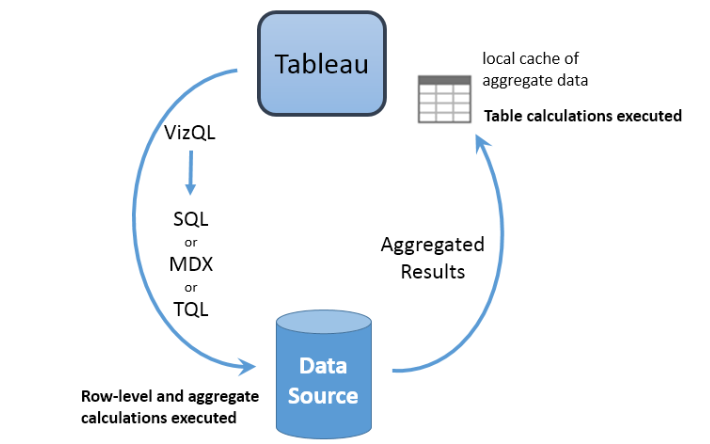
\includegraphics[width=0.8\linewidth]{Figures/TableCalculation.png}
    \end{center}
    \caption{Execution flow of a table calculation \protect\cite{LearningTableau}.}
    \label{fig:TableCalculation}
\end{figure}

Tableau gives the user the possibility to use a great variety of operations, but it's also possible to write a custom table calculation, such as:

\begin{itemize}
    \item Computing the running total.
    \item Computing time variance in both absolute values and percentage.
    \item Computing the moving and percentile average.
    \item Ranking or sorting according to specific functions.
\end{itemize}

\subsubsection{Analysis}

Another innovative feature present in Tableau is the possibility to make statistical analyses through mathematical models built-in or use algorithms written in \textbf{R, Python or MatLab} \cite{LearningTableau}. The main built-in models usable in Tableau are:

\begin{itemize}
    \item \textbf{Trend lines}: each trend line added to a chart represents a regression, which Tableau builds according to linear, logarithmic, exponential or polynomial models.
    \item \textbf{Forecasting}: in case of the visualization of a time series, it's possible to use the "exponential smoothing" method to compute future values according to an exponential function weighing current value and past values' average; Tableau can also recognize periodic patterns in time series.
    \item \textbf{Clustering}: Tableau uses K-Means algorithm to classify the data on the chosen variables and gives the user the possibility to change the value of K, that is the number of total clusters.
\end{itemize}

\section{Tableau Server}

\textbf{Tableau Server} is a server application used to contain data and metadata of sources and shared workbooks. Through an Access Control List based on accounts, Tableau server allows users to view, interact, download, share and edit a worksheet without the need install Tableau Desktop. Additionally, through the sharing of an already present data source, a user can create new worksheets without installing the correspondent drivers.

\subsection{Tableau Embedded}

Tableau Server offers the possibility to embed worksheets in a web application using Tableau JavaScript API, which allows for:

\begin{itemize}
    \item Viewing and interacting with the shared view.
    \item Loading and resizing the view dynamically.
    \item Download the view as a PDF or an image.
\end{itemize}

Corresponding user credentials would be required to view the shared charts and plots, but it's possible to use Tableau's \textit{Trusted Authentication} to authenticate the server hosting the application to allow all the web app user access to it.
\chapter{Security}

As the main goal of our whole architecture is to extract information and actionable insights from data, there needs to be a tight security customized to our infrastructure in order to protect that valuable data.
To protect the data we use several layers of security, some seen commonly in other systems, some peculiar to our stack.
\newline
Firstly, access to the cluster internal network must be denied to every outside request but for few selected ports on a front end machine, this is obtained through standard ACLs.
The only connections available to both Clients and Developers must be through secure channels (HTTPS\footnote{HTTPS: HyperText Transfer Protocol over Secure Socket Layer, standard protocol for secure web pages}, SSH\footnote{SSH: Secure SHell, protocol for remote controls of Command Line Interfaces}, FTPS\footnote{FTPS: File Transfer Protocol over Secure Socket Layer, self explanatory}).
\newline
Secondly, the author of the request that passed through ACL must be authenticated by an authentication provider such as LDAP\footnote{LDAP: Lightweight Directory Access Protocol, a standard protocol  for accessing distributed directory information services over an intranet} or Kerberos, and then authorised to follow through with its request with respect to its identity.
\newline
Thirdly, a service must provide Auditing for all requests, whether denied or allowed so that actions and their consequences can be attributed to their authors.

\pagebreak

\section{Knox}

\textbf{Apache Knox} \cite{knox_doc} is an Application Gateway, part of the Hadoop environment, that offers several security functionalities for a Hadoop Cluster right after the first layer provided by the ACL and acts as a Reverse Proxy with policy enforcement.
\subsection{Authentication and Acces Control}
The Knox gateway exposes a single secure access point for all REST\footnote{REST: REpresentational State Transfer, a type of stateless software architecture whose aim is to provide access to resource in an interoperable way through the web} APIs and HTTP interactions with the cluster.\newline
All client requests to RESTful APIs and webUIs are sent to Knox through HTTPS with their respective user credentials, Knox authenticates the user with the help of an authentication provider such as Kerberos or LDAP, then thanks to an authorisation provider offers Access Control to the single services, if access is allowed, the request is routed to the target service.
Failed authentication, failed authorisation and successful requests are all logged, providing a first layer of Auditing.
\subsection{Structure}
The two main components of Knox are the Topology files and the services' files.
\newline
The Topology is an XML file representing a gateway, it is divided in two main sections: the gateway/provider section and the service section; the former section is comprised of the configuration settings enforced by the gateway while providing access to the Hadoop cluster, these settings describe the services that fulfil various roles such as the Authentication provider, the Federation or Single Sign-On provider, the Authorisation provider and the Hostmap which maps external to internal node hostnames.
The service section provides a list of services accessible from the gateway and the address in the cluster where they can be found.
\newline
For each service listed in the Topology, two files are needed: 
\begin{itemize}
	\item service.xml, which defines the high level URL patterns to be exposed by the gateway for that service, such as the shape of the incoming request to be matched.
	\item rewrite.xml, which defines regular expression through which the request must be rewritten before being sent to the cluster internal service.
\end{itemize}
Knox comes packaged with several files for common Hadoop services and permits the definition of custom ones. 

\section{Ranger}

\textbf{Apache Ranger} \cite{ranger_doc}is a comprehensive framework to manage data security, authorisation, data governance and audit in Hadoop clusters.

Ranger provides a centralised security administration able to manage in one place most of the security related tasks inside the cluster, with a high granularity thanks to its customization for Hadoop services.

Plain authentication is accepted, and can be used if a previous layer has already authenticated the user (such as Knox), otherwise Ranger supports LDAP and Unix Authentication.

\subsection{Authorisation}
A request coming from within the cluster to a service for which Ranger is enabled, provided previous authentication, must be authorised by Ranger according to precise policies specific to the service.

Ranger supports several plugins for the major services containing critical data, such as HDFS, HBase, Hive and YARN plus a selection of other services that process or ingest data and interact with the former four.
\newline Authorization can be granted through policies to certain groups or users to services altogether (access-authorization) or to specific resources inside them (resource-classification).
\newline
To exemplify the granularity provided by Ranger here's presented an image depicting a policy on Hive that allows only \textbf{SELECT} requests from a restricted group on certain rows of a specific table in a database.

\begin{figure}
	\centering
	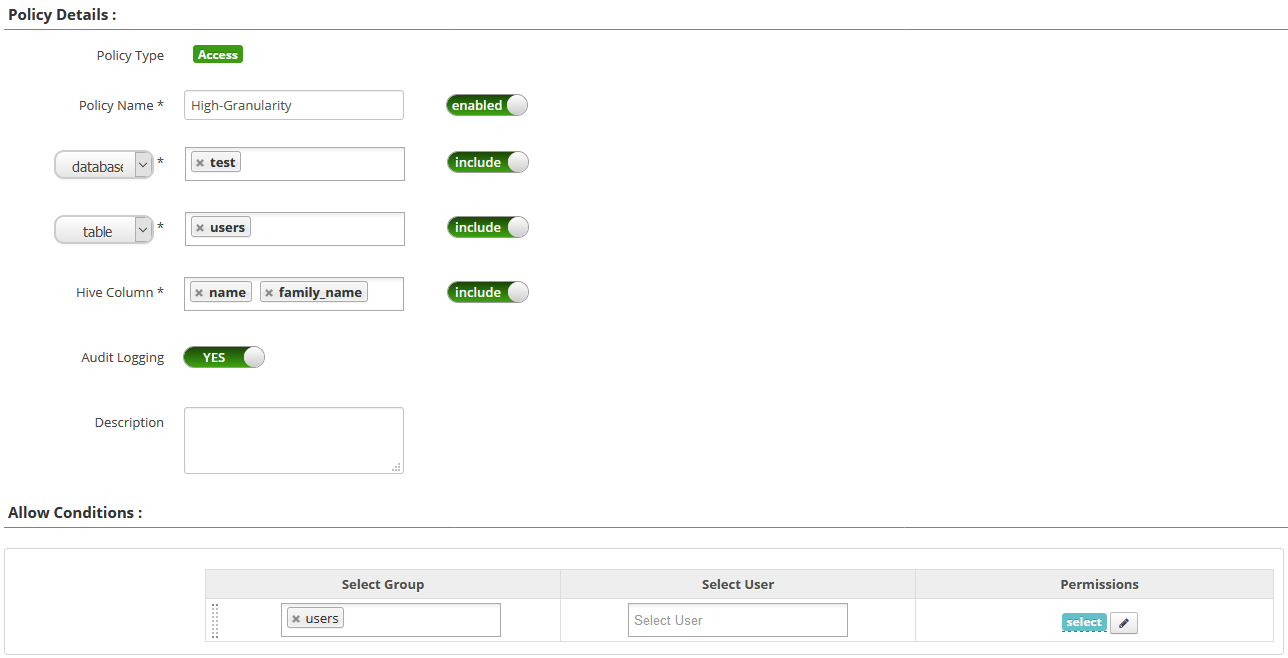
\includegraphics[scale=0.5]{Figures/policy.png}
	\decoRule
	\caption[Infrastructural Stack]{A Ranger policy for Hive}
	\label{fig:Policy}
\end{figure}

\subsection{Tag Based Policies and Persistence}

New versions of Ranger support a new type of Policy based on Tags; Tags can be associated with single resources inside other services, providing those resources the same kind of policy without having to specify it, this makes it easier to separate access-authorization and resource-classification and to manage the latter.\newline
Tags and related information are stored in the Tag Store, while a TagSync process is responsible for synchronisation with other services using Tags such as Apache Atlas.
\newline
Policies and users are stored in a MySQL database on one of the hosts' file system, a synchronisation process is designated with managing users between Ranger, Ambari and other security services such as LDAP/Active Directory.\newline
Auditing of all accesses are stored on HDFS directly or through Apache Solr, a fast search engine.
\chapter{Air Traffic monitoring: a use case}

\section{Introduction}

Air traffic monitoring can be considered a practical use case for the infrastructure described in the previous chapters, being characterised by the Big Data 3 Vs, as there are more than 5000 aircrafts flying any time (Volume), each one of which is transmitting data via transponder signals once every few seconds (Velocity) and, for each data source, data formats can be wildly different from one another, while, additionally, raw data transmitted by aircrafts can be used in conjunction with other kinds of data, such as weather and social networks, for deeper analytics (Variety).

\section{Infrastructure overview}

The infrastructure bones have been built with a series of Virtual Machines provisioned in the Azure Pack Cloud-On-Premise environment provided by the VarGroup Data Center located in Empoli (FI). There are, in total, seven VMs mounting CentOS 7 and the following specifications:
\\
% Table with specifications
\\
All of these VMs are part of an \textbf{Hortonworks} cluster featuring HDP 2.6.1, deployed via Ambari Blueprint interface through an aptly made scripting suite to automate machine preparation. As additional software used, other than Hortonworks Hadoop distribution, which includes HDFS, YARN, Spark 2, Hive, Kafka, Zookeeper, Ranger, Knox and NiFi, \textbf{Flink 1.4} binaries have been compiled from sources targeting Hortonworks hadoop version and installed for usage on top of YARN, while a Cassandra cluster has been installed on the four slave nodes.

The cluster has been made secure by the gatekeeping provided by Knox and the fact that access is only possible through the front-end machine, accessible only via passwordless SSH by operators and developers, which additionally implements iptables as firewall for prevent access to unwanted ports from external request.

\textbf{Note:} additional 10 VMs have been provisioned in the same environment for a MongoDB cluster, used as an additional data sink after Flink processing.

\section{Deployment \& Operations}

As mentioned, the virtualised cluster has been provisioned in a \href{https://www.microsoft.com/it-it/cloud-platform/windows-azure-pack}{Azure Pack Cloud-On-Premise} environment, which allows to automate the virtual machines creation and management through \textbf{Azure Powershell} tools and its set of \textbf{cmdlets}\footnote{A \textit{cmdlet} is a lightweight command that is used in the Windows PowerShell environment within the context of automation scripts that are provided at the command line, executing an action and returning a Microsoft .NET Framework object to the next command in the pipeline.} to create, remove and, in general, manage Virtual Machine and their allocated resources.

\subsection{Hadoop Cluster Deployment}

After the virtualised cluster creation, Hadoop and other cluster services need to be installed. In order to do that, as a way to streamline a cluster installation, \textbf{Hortonworks HDP 2.6.1} hadoop distribution has been chosen (with Hadoop 2.7.3.2.6.1.0-129, from Hortonworks repositories), rather than installing all of the hadoop services one-by-one. When it comes to the cluster installation, HDP main feature is \textbf{Apache Ambari}\footnote{\href{https://ambari.apache.org/}{Apache Ambari} is a software for provisioning, managing, and monitoring Apache Hadoop clusters, providing an intuitive, easy-to-use Hadoop management web UI backed by its RESTful APIs.} and its Blueprint REST interface for a cluster installation which can be made through a single REST call. For this very reason, a script suite called \textbf{hw-install}\footnote{\href{https://github.com/fedexist/hw-install}{hw-install} is Python 2.7 script suite to automate an Hortonworks cluster installation} has been developed to take advantage of that functionality and automate the cluster preparation and configuration, before the actual deployment.

\textbf{hw-install} is composed of two main packages: \texttt{hw\_install} and \texttt{\justify{hw\_add\_new\_host}}, while the first one handles the installation of an entire cluster given a proper configuration in YAML format, the second one handles the preparation of a new host to be added to an existing cluster via the Ambari Server UI.

Both packages use the same core components for the preparation of cluster hosts:

\begin{itemize}
    \item Set-up of \textbf{passwordless SSH} communication between hosts with a common RSA key identifying the user executing \texttt{hw\_install}, by default and as recommended by Hortonworks Setup guide the user is \textbf{root};
    \item Increase of the number of \textbf{file descriptors} available in the system;
    \item Installation of the \textbf{NTP} (Network Time Protocol) service, for hosts time synchronization;
    \item Disabling of \textbf{firewall and SELinux}, in order to allow hosts to communicate freely between each other;
    \item Set-up of \textbf{hostnames, FQDNs}\footnote{Fully Qualified Domain Name} \textbf{and DNSs};
    \item Installation on the selected host of the \textbf{Ambari Server}, together with the Ambari Agents, on all of the hosts
\end{itemize}

In addition, \texttt{hw\_install} actually uses \textbf{Ambari Blueprint} interface, passing the configuration file containing the needed services and their per-component configuration, if any (in absence of this per-component configuration, Ambari will apply default values), and then making a REST call to the Ambari Server which will take care of the installation of the needed components on the selected hosts.
\\\\
An example of a configuration file is:

\begin{minted}[breaklines, breakafter="ambari/"]{YAML}
cluster-name: cluster_name
blueprint-name: blueprint_name
ambari-repo: http://public-repo-1.hortonworks.com/ambari/centos7/2.x/updates/2.5.1.0/ambari.repo
Blueprints: # HDP version to be installed
    stack_name: HDP
    stack_version: 2.6
ambari-server: # Host where Ambari Server will be installed
    IP: 192.168.1.1
    FQDN: master.localdomain
hosts: # Other hosts in the cluster
    - IP: 192.168.1.2
      FQDN: slave.localdomain
host-groups:
    - name: master
    hosts: # Hosts belonging to the 'master' host group
        - fqdn: master.localdomain
    components: # Services to be installed in 'master' host group
        - name: YARN_CLIENT
        - name: HDFS_CLIENT
        - name: HIVE_SERVER
        - name: HIVE_METASTORE
        - name: NAMENODE
        - name: ZOOKEEPER_CLIENT
        - name: RESOURCE_MANAGER
        - name: WEBHCAT_SERVER
        - name: ZOOKEEPER_SERVER
        - name: AMBARI_SERVER
.....
\end{minted}

Once a cluster has been installed, it's easy to add another host to the cluster, using \texttt{hw\_add\_new\_host}: after adding the appropriate \texttt{new-hosts} entries to the configuration file of the cluster, executing this script allows to set-up the host before manually adding it to the cluster from the Ambari Server UI, where it's possible to select the new services to be installed.

\subsection{Flink \& Cassandra Deployment}

For the current use case, it's been chosen to use Flink running on top of YARN, so that there's no need to set up a standalone Flink cluster with its own configuration. In order to use Flink, it's then necessary to download the sources of the needed version, 1.4.0 in this case, and compile it against the hadoop version which was installed and selecting, if needed, the Scala version which is going to be used while developing the Flink applications.\\
\\
Cassandra deployment is rather straightforward, since, starting from a common \texttt{\justify{cassandra.yaml}} configuration file where all of the nodes have been noted as cluster \texttt{seeds}, it's possible, after importing its repository, to install it directly from CentOS package manager as a system daemon/service.

\subsection{Deployed Software \& Versions}

To sum up, the cluster has been provisioned with HDP 2.6.1, which includes:
\begin{itemize}
    \item Hadoop 2.7.3.2.6.1.0-129 (HDFS, YARN and MapReduce),
    \item Tez 0.7.0,
    \item Hive 1.2.1000, 
    \item ZooKeeper 3.4.6,
    \item Kafka 0.10.1,
    \item Knox 0.12.0,
    \item Ranger 0.7.0,
    \item Spark 2.1.1,
    \item NiFi 1.2.0,
    \item Registry 0.3.0,
    \item Slider 0.92.0.
\end{itemize}

In addition, it's been used Flink 1.4.0 for Scala 2.11 compiled from sources against hadoop 2.7.3.2.6.1.0-129 and Cassandra 3.11.
\\
\\
The cluster is composed of seven machines:
\begin{itemize}
    \item \texttt{frontend}, with Knox and a Nginx reverse proxy installed, used as single point of entry for developers and cluster operators to access cluster services via SSH tunneling. Specifications: 1 core, 512 MB of RAM.
    \item \texttt{master-1}, one of the two master components of the cluster, with an HDFS Namenode, a Zookeeper Server, a Registry MySQL database, a Kafka Broker, Hive Metastore and HiveServer 2 Interactive (support for Hive LLAP daemons), Ranger Admin and UserSync, a NiFi node and Spark2 History Server. Specifications: 4 core, 12 GB of RAM.
    \item \texttt{master-2}, the other master component of the cluster, with the YARN Resource Manager and App Timeline Server, HDFS Secondary Namenode, a Zookeeper Server, a WebHCat Server and HiveServer2 for Hive, a Kafka Broker, a Nifi node, MapReduce2 History Server and Flink binaries. Specifications: 4 core, 12 GB of RAM.
    \item Four slave machines, slave-1, slave-2, slave-3, slave-4, with a YARN Node Manager, HDFS DataNode and Cassandra nodes. Specifications: 4 core, 6 GB of RAM.
\end{itemize}

\section{Development}

\subsection{Ingestion}

\subsection{Processing}

\subsection{Serving \& Security}

\subsection{Accessory Services}

\subsection{Visualization}

%----------------------------------------------------------------------------------------
%	THESIS CONTENT - APPENDICES
%----------------------------------------------------------------------------------------

%\appendix % Cue to tell LaTeX that the following "chapters" are Appendices

% Include the appendices of the thesis as separate files from the Appendices folder
% Uncomment the lines as you write the Appendices

%% Appendix A

\chapter{Frequently Asked Questions} % Main appendix title

\label{AppendixA} % For referencing this appendix elsewhere, use \ref{AppendixA}

\section{How do I change the colors of links?}

The color of links can be changed to your liking using:

{\small\verb!\hypersetup{urlcolor=red}!}, or

{\small\verb!\hypersetup{citecolor=green}!}, or

{\small\verb!\hypersetup{allcolor=blue}!}.

\noindent If you want to completely hide the links, you can use:

{\small\verb!\hypersetup{allcolors=.}!}, or even better: 

{\small\verb!\hypersetup{hidelinks}!}.

\noindent If you want to have obvious links in the PDF but not the printed text, use:

{\small\verb!\hypersetup{colorlinks=false}!}.

%\include{Appendices/AppendixB}
%\include{Appendices/AppendixC}

%----------------------------------------------------------------------------------------
%	BIBLIOGRAPHY
%----------------------------------------------------------------------------------------

\printbibliography[heading=bibintoc]

%----------------------------------------------------------------------------------------

\end{document}  
